%%%%%%%%%%%%%%%%%%%%%%%%%%%%%%%%%%%%%%%%%%%%%%%%%%%%%%%%%%%%%%%%%%%%%%%%%
% Antes de correr el código:
% 1. Ingresar al Menu
% 2. Cambiar la opción "Compiler" a XeLaTeX
% 3. Cambiar la opción "TeX live version" a 2020 (opacidad de la imagen)
%%%%%%%%%%%%%%%%%%%%%%%%%%%%%%%%%%%%%%%%%%%%%%%%%%%%%%%%%%%%%%%%%%%%%%%%%
\documentclass[10pt]{article}
\usepackage[T1]{fontenc}
\usepackage[utf8]{inputenc}
\usepackage[english]{babel}
\usepackage{listings}
\lstset{language=R}
\usepackage[a4paper]{geometry}
\usepackage[dvipsnames]{xcolor}
\usepackage[framemethod=TikZ]{mdframed}
\usepackage{graphicx,tikz}
\usepackage{array}
\usepackage{float}
\usepackage{tocloft}
\setlength{\cftsecnumwidth}{2em}
\usepackage{xspace}
\usepackage{tcolorbox}
\tcbuselibrary{listings}

\newtcblisting{cc}{
  listing only,
  nobeforeafter,
  after={\xspace},
  hbox,
  tcbox raise base,
  fontupper=\ttfamily,
  colback=lightgray,
  colframe=lightgray,
  size=fbox
  }

\geometry{top=2.54cm, bottom=2.54cm, left=2.54cm, right=2.54cm}

\usepackage{url}
\usepackage{lipsum} 
\usepackage{wrapfig}
\usepackage{subcaption}
\usepackage{multicol}

%==========================================
%======     FUENTE PARA CÓDIGOS      ======
%==========================================
\definecolor{codegreen}{rgb}{0,0.6,0}
\definecolor{codegray}{rgb}{0.1,0.1,0.1}
\definecolor{backcolour}{rgb}{0.98,0.98,0.98}

\lstdefinestyle{mystyle}{
  backgroundcolor=\color{backcolour},   
  commentstyle=\color{codegreen},
  keywordstyle=\color{blue},
  numberstyle=\tiny\color{codegray},
  stringstyle=\color{codegreen},
  basicstyle=\ttfamily\footnotesize,
  breakatwhitespace=false,         
  breaklines=true,                 
  captionpos=b,                    
  keepspaces=true,                 
  numbers=left,                    
  numbersep=5pt,                  
  showspaces=false,                
  showstringspaces=false,
  showtabs=false,                  
  tabsize=2
}

%==========================================
%==========     ESTILO TITLE     ==========
%==========================================
\newcommand{\City}[1]{\def\City{#1}}

\makeatletter         
\renewcommand\maketitle{
\begin{flushleft}
{\textcolor{black}{\huge \bfseries \@title }}\\[1ex]
\rule{\textwidth}{0.6pt}\\
\end{flushleft}
\vspace{-0.5cm}

\begin{flushleft}
\textcolor{black}{{\large  \@author} }\\[2ex]
\end{flushleft} } % Note the extra }
\makeatother

%==========================================
%==========    ESTILO CAPTION    ==========
%==========================================
\usepackage{caption}
\captionsetup[table]{name=Tabla ,textfont={it}, labelfont={bf},
                     justification=centering,
                     width =\dimexpr \textwidth-0.5cm\relax}
\captionsetup[figure]{textfont={it}, labelfont={bf},
                      justification=centering, skip=2pt,
                      belowskip=-5pt}
                      
%==========================================
%==========     ESTILO ITEM      ==========
%==========================================
\renewcommand{\labelitemi}{$\bullet$} 
\renewcommand{\labelitemii}{$\circ$} 
\renewcommand{\labelitemiii}{$\cdot$} 

%==========================================
%===    LINKS (Agregar Hyperlinks)     ====
%==========================================
\usepackage[style=apa,
            urldate=long]{biblatex} 
\addbibresource{Bib.bib}

\DeclareSourcemap{
  \maps[datatype=bibtex]{
    \map{
      \step[fieldsource=note, final]
      \step[fieldset=addendum, origfieldval, final]
      \step[fieldset=note, null]}
      }
}

\DefineBibliographyStrings{english}{urlseen = {Accessed }    
}

\usepackage[colorlinks=true,linkcolor=RoyalBlue,
            citecolor=RoyalBlue,urlcolor=RoyalBlue]{hyperref}

%==============================================================
%==============================================================
\title{ }

%%%%%%%%%%%%%%%%%%%%%%%%%%%%%%%%%%%%%%%%%%%%%%%%%%%%%%%%%%%%%%%
%%%%%%%%%%%%                 INICIO                %%%%%%%%%%%% 
%%%%%%%%%%%%%%%%%%%%%%%%%%%%%%%%%%%%%%%%%%%%%%%%%%%%%%%%%%%%%%%
\begin{document}

\begingroup
\let\clearpage\relax % prevent extra page breaks
\thispagestyle{empty}
\begin{center}
{\huge \bfseries Universidad de los Andes}

\vspace{25pt}
{\LARGE \bfseries Departamento de Ingeniería de Sistemas}

\vspace{15pt}

\includegraphics[width=100pt]{images/logo.png} 

\vspace{35pt}
{\LARGE \bfseries Laboratorio \#2: Análisis De Protocolos De La Capa De Aplicación}
\vspace{55pt}

{\Large \bfseries ISIS3204 - Infraestructura de Comunicaciones}


\vspace{100pt}
{\Large \bfseries Grupo 3: }

\end{center}

\begin{flushleft}
  \setlength{\parskip}{0pt}
  \setlength{\itemsep}{0pt}
  \hspace*{4cm}\large\bfseries Juan Esteban Quiroga - 202013216

  \hspace*{4cm}\large\bfseries Juan Manuel Rodriguez - 202013372

  \hspace*{4cm}\large\bfseries Andres Felipe Ortiz - 201727662
\end{flushleft}

\begin{center}
\vspace{60pt}

\Large\bfseries 2025-10
\end{center}

\mbox{}
\endgroup

\clearpage

\tableofcontents
\clearpage


\renewcommand{\thesection}{\arabic{section}}
\section*{Introducción}
\addcontentsline{toc}{section}{Introducción}
En este laboratorio configuramos y probamos algunos servicios de red: DNS, HTTP/HTTPS, FTP, VoIP y RTMP, usando una topología a pequeña escala. Con Wireshark analizamos la conectividad de estos servicios en dicha red. Este laboratorio nos ayudó a entender la interacción de protocolos importantes que soportan la comunicación en redes de computadores. En la figura 1 mostramos las IPs estáticas que usamos para este laboratorio. (Es importante que estas IPs no sean dinamicas por DHCP ya que esto asegura direccionamiento constante y facilidad de configuración stable en la red.) La asignación de direcciones inició en $172.20.10.5$ porque el gateway de la red es el hotspot del iPhone en $172.20.10.1$, dejando libres las direcciones previas para posibles equipos de infraestructura y evitando conflictos.


\begin{figure}[H]
    \centering
    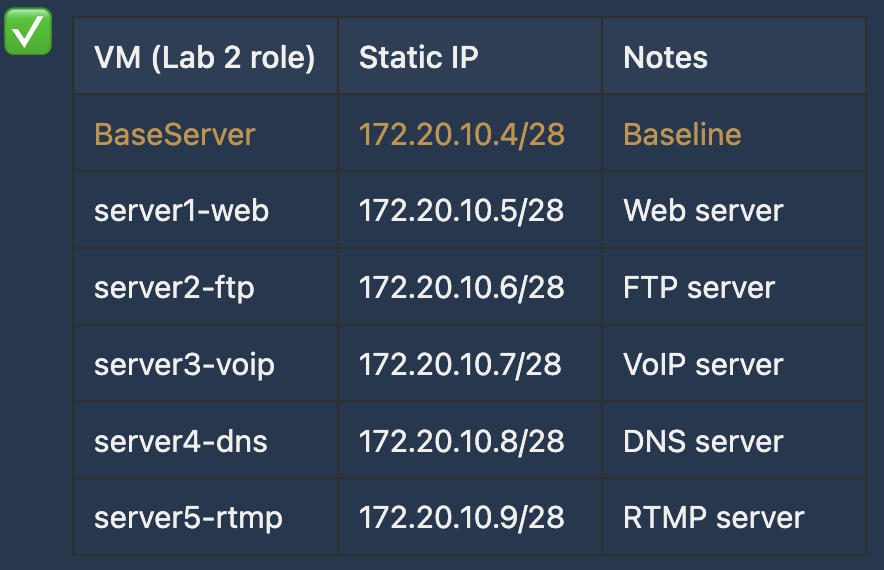
\includegraphics[width=0.55\textwidth]{lab-02-screenshots/server-ips.png}
    \caption{Configuración de IPs estáticas}
\end{figure}


%==============================================================
%=====================   8.1   ================================
%==============================================================
\renewcommand{\thesection}{8.\arabic{section}}
\setcounter{section}{0}
\section{Prueba ping}

En esta sección se verifica la conexión básica entre el cliente y los servidores DNS y FTP mediante pings con el protocolo ICMP, asegurando la conectividad antes de analizar los demás protocolos.

\subsection{Prueba de conectividad al servidor DNS}

Desde el cliente se enviaron pings (echo requests ICMP ) al servidor DNS utilizando su dirección IP (\textbf{172.20.10.8}). El tráfico generado se capturó y se guardó en el archivo \textcolor{blue}{\texttt{Ping\_DNS\_IP.pcap}}. El archivo fue abierto en Wireshark y se aplicó el filtro icmp para observar únicamente los paquetes de ping. Se registraron la dirección IP de origen, dirección IP de destino, dirección MAC de origen y dirección MAC de destino en las tramas capturadas.

\begin{figure}[H]
    \centering
    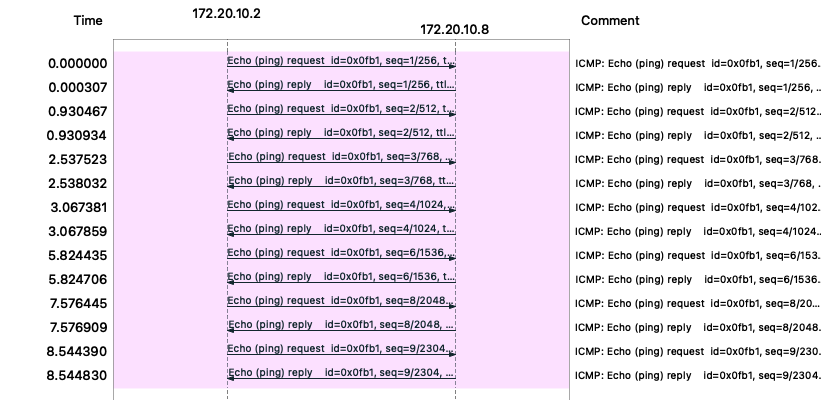
\includegraphics[width=0.85\textwidth]{lab-02-screenshots/8.1-DNS-flow}
    \caption{Flujo de packets en DNS ping}
\end{figure}


\begin{figure}[H]
    \centering
    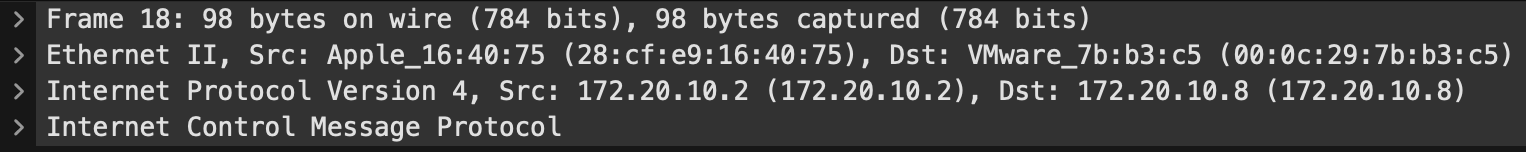
\includegraphics[width=0.85\textwidth]{lab-02-screenshots/8.1-DNS-data}
    \caption{Evidencia de IPs y MACs origen/destino}
\end{figure}

\begin{figure}[H]
    \centering
    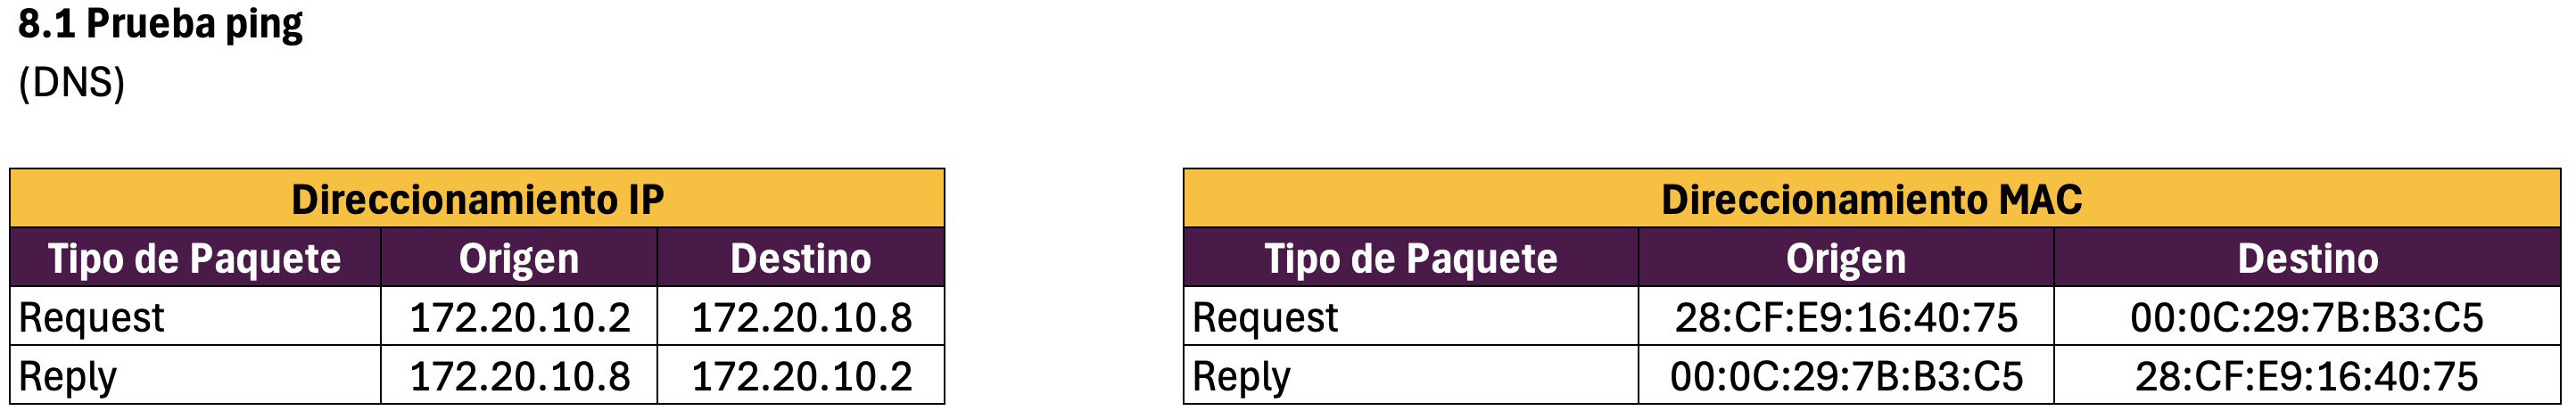
\includegraphics[width=0.85\textwidth]{lab-02-screenshots/8.1-DNS-ping-table}
    \caption{Tabla de IPs y MACs origen/destino}
\end{figure}


\subsection{Prueba de conectividad al servidor FTP}

Desde el cliente se enviaron pings al servidor FTP utilizando su dirección IP. El tráfico generado se capturó y se guardó en el archivo \textcolor{blue}{\texttt{Ping\_FTP\_IP.pcap}} El archivo fue analizado en Wireshark con el filtro icmp. Se identificaron las direcciones IP y MAC correspondientes a los paquetes de solicitud y respuesta.

\begin{figure}[H]
    \centering
    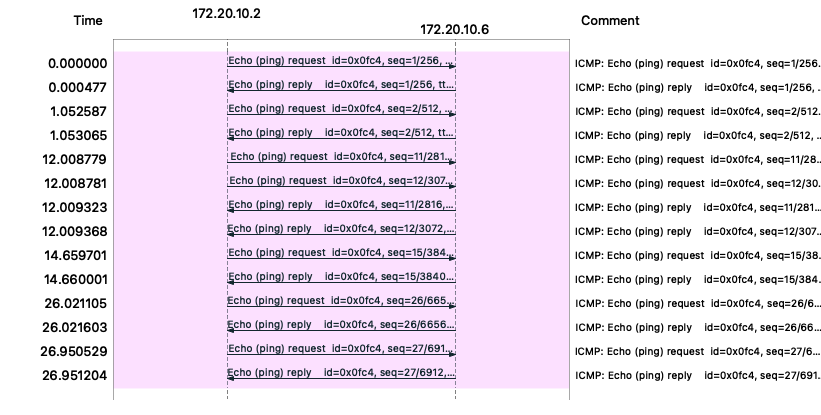
\includegraphics[width=0.85\textwidth]{lab-02-screenshots/8.1-FTP-flow}
    \caption{Flujo de packets en FTP ping}
\end{figure}


\begin{figure}[H]
    \centering
    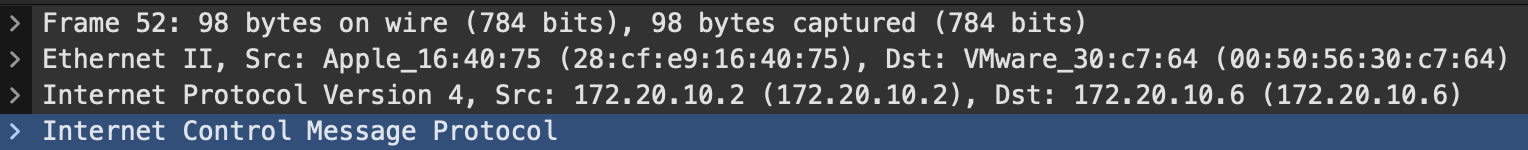
\includegraphics[width=0.85\textwidth]{lab-02-screenshots/8.1-FTP-data}
    \caption{Evidencia de IPs y MACs origen/destino}
\end{figure}

\begin{figure}[H]
    \centering
    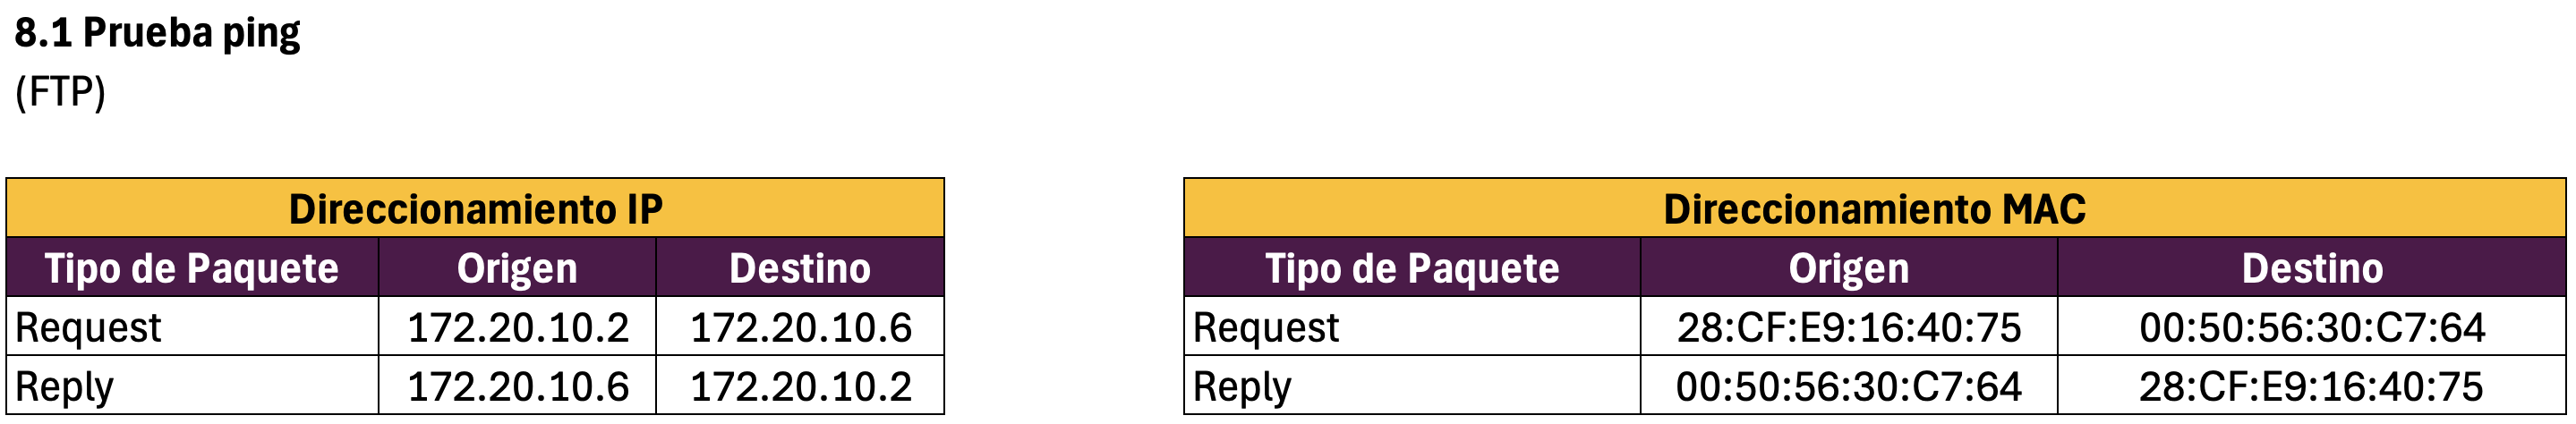
\includegraphics[width=0.85\textwidth]{lab-02-screenshots/8.1-FTP-ping-table}
    \caption{Tabla de IPs y MACs origen/destino}
\end{figure}

\begin{figure}[H]
    \centering
    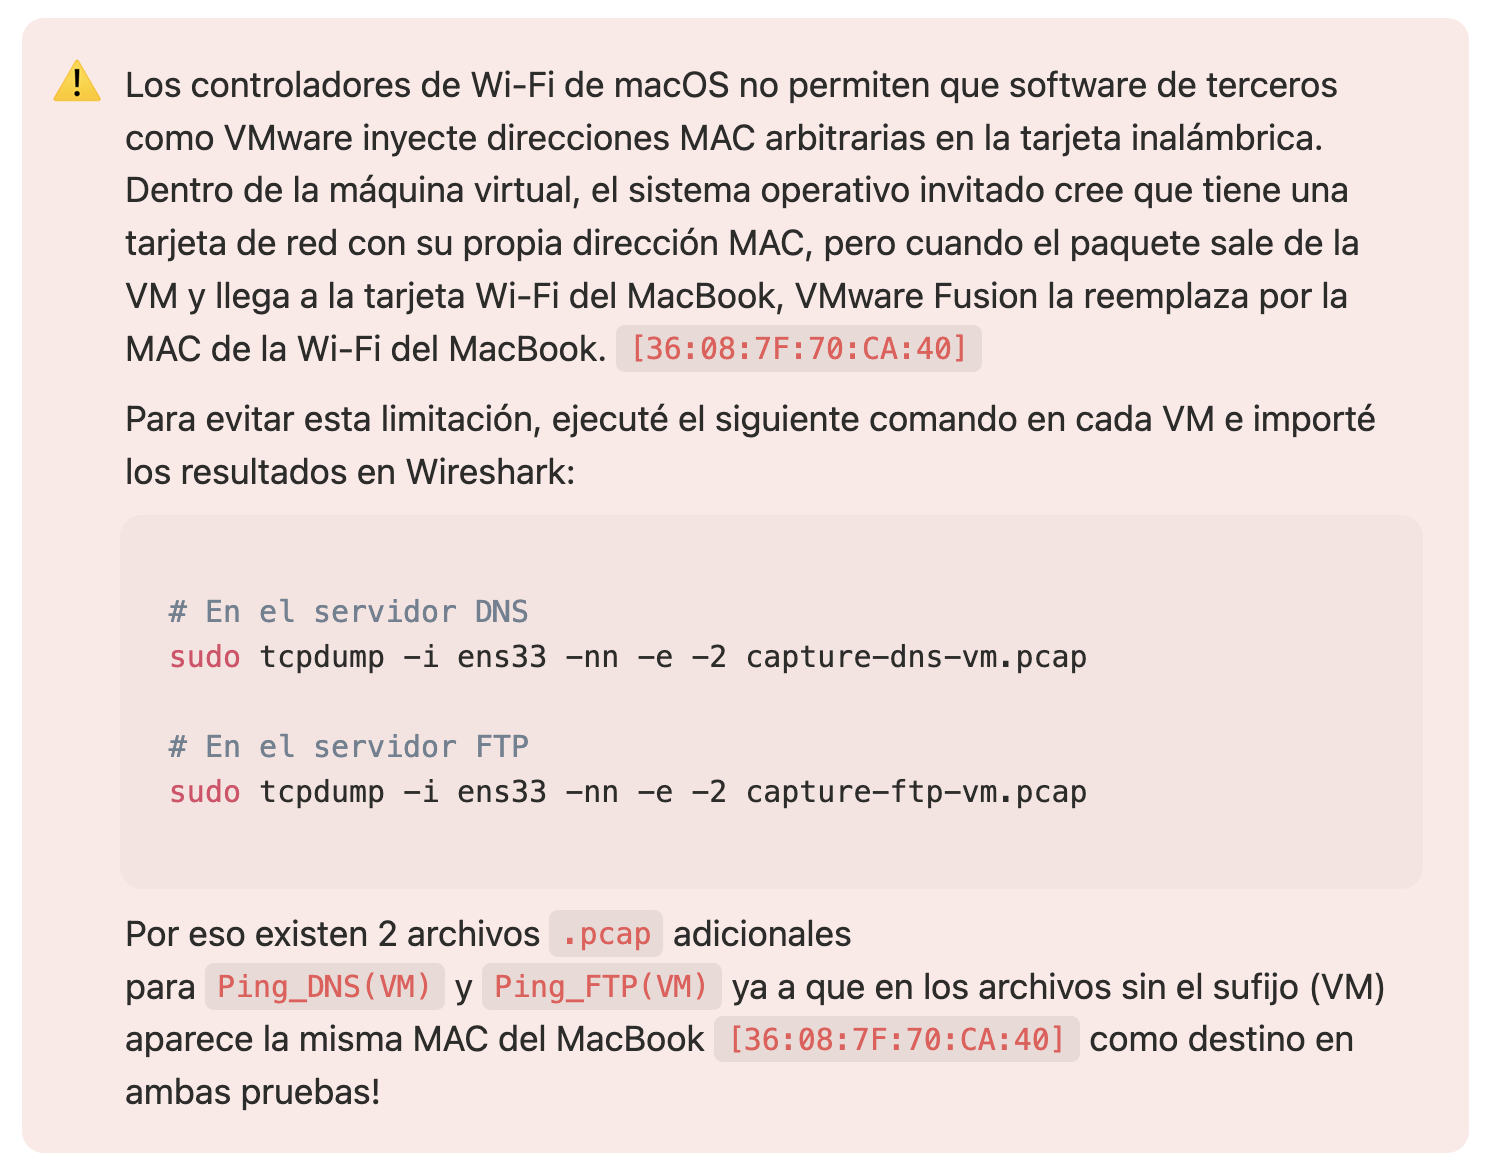
\includegraphics[width=0.85\textwidth]{lab-02-screenshots/8.1-disclaimer}
\end{figure}

%==============================================================
%=====================   8.2   ================================
%==============================================================
\renewcommand{\thesection}{8.\arabic{section}}
\section{Análisis de tráfico del Servicio DNS}

En esta sección se analiza el servicio DNS, que traduce nombres de dominio en direcciones IP para facilitar la comunicación en la red. Se genera y captura tráfico con Wireshark, identificando consultas y respuestas, así como el protocolo de transporte y los puertos utilizados al acceder a un servidor web por IP y por nombre de dominio.


Cuando un cliente necesita comunicarse con un dominio, primero envía al servidor DNS una consulta de tipo \textit{A} para obtener su dirección IPv4 y, en paralelo, una consulta de tipo \textit{AAAA} para la dirección IPv6. El servidor responde con los registros correspondientes, que el cliente almacena en caché. Con la IP resuelta, el cliente ya puede establecer la comunicación (ej. enviar un ping) directamente al servidor destino.  

\subsection{Prueba de conectividad al Servidor Web (IP)}
Cuando se accedió al servidor escribiendo directamente su dirección IP en el ping request, la conexión se estableció de inmediato ya que no fue necesario consultar al DNS y en la captura se observó únicamente tráfico ICMP entre cliente y servidor. El tráfico generado se capturó y se guardó en el archivo \textcolor{blue}{\texttt{Ping\_WEB\_IP.pcap}} El archivo fue analizado en Wireshark con el filtro icmp.

\begin{figure}[H]
    \centering
    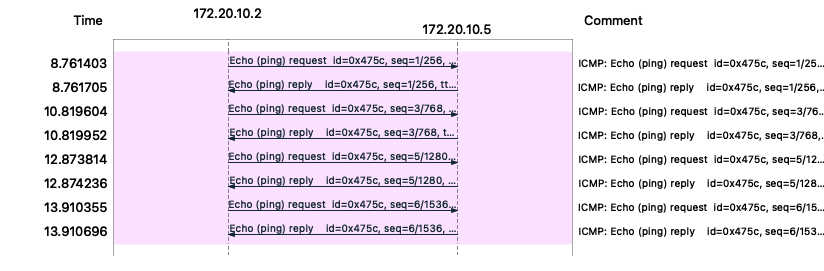
\includegraphics[width=0.85\textwidth]{lab-02-screenshots/8.2-WEB-IP-flow}
    \caption{Flujo de packets en WEB IP ping}
\end{figure}


\begin{figure}[H]
    \centering
    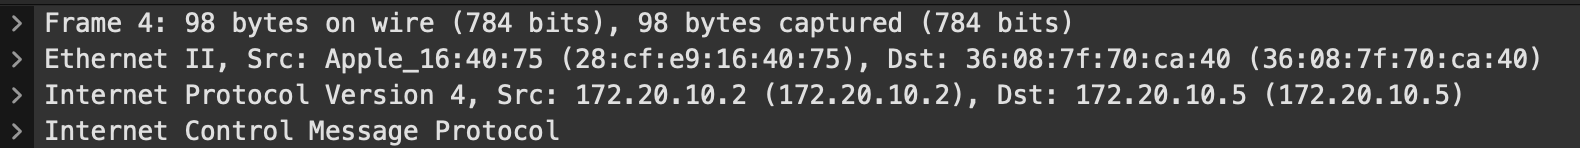
\includegraphics[width=0.85\textwidth]{lab-02-screenshots/8.2-WEB-IP-data}
    \caption{Evidencia de IPs, MACs, y puertos origen/destino}
\end{figure}

\textbf{En esta prueba, no hay resolución DNS.}

\subsection{Prueba de conectividad al Servidor Web (URL)}
Cuando se accedió al servidor utilizando su nombre de dominio en la solicitud de ping, el cliente primero realizó consultas de tipo A y AAAA al servidor DNS para obtener la dirección IP correspondiente. Una vez resuelta, se estableció la comunicación con el servidor y en la captura se observó inicialmente el tráfico DNS seguido por el intercambio ICMP entre cliente y servidor. El tráfico generado se capturó y se guardó en el archivo \textcolor{blue}{\texttt{Ping\_WEB.pcap}}, el cual fue analizado en Wireshark aplicando filtros para DNS e ICMP.


\begin{figure}[H]
    \centering
    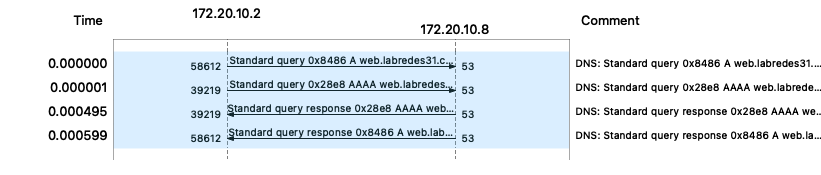
\includegraphics[width=0.85\textwidth]{lab-02-screenshots/8.2-WEB-flow}
    \caption{Flujo de packets en WEB Domain ping}
\end{figure}


\begin{figure}[H]
    \centering
    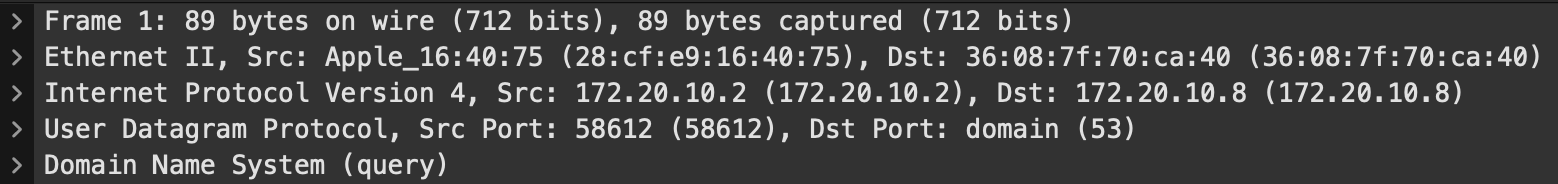
\includegraphics[width=0.85\textwidth]{lab-02-screenshots/8.2-WEB-data}
    \caption{Evidencia de IPs, MACs, y puertos origen/destino}
\end{figure}


\begin{figure}[H]
    \centering
    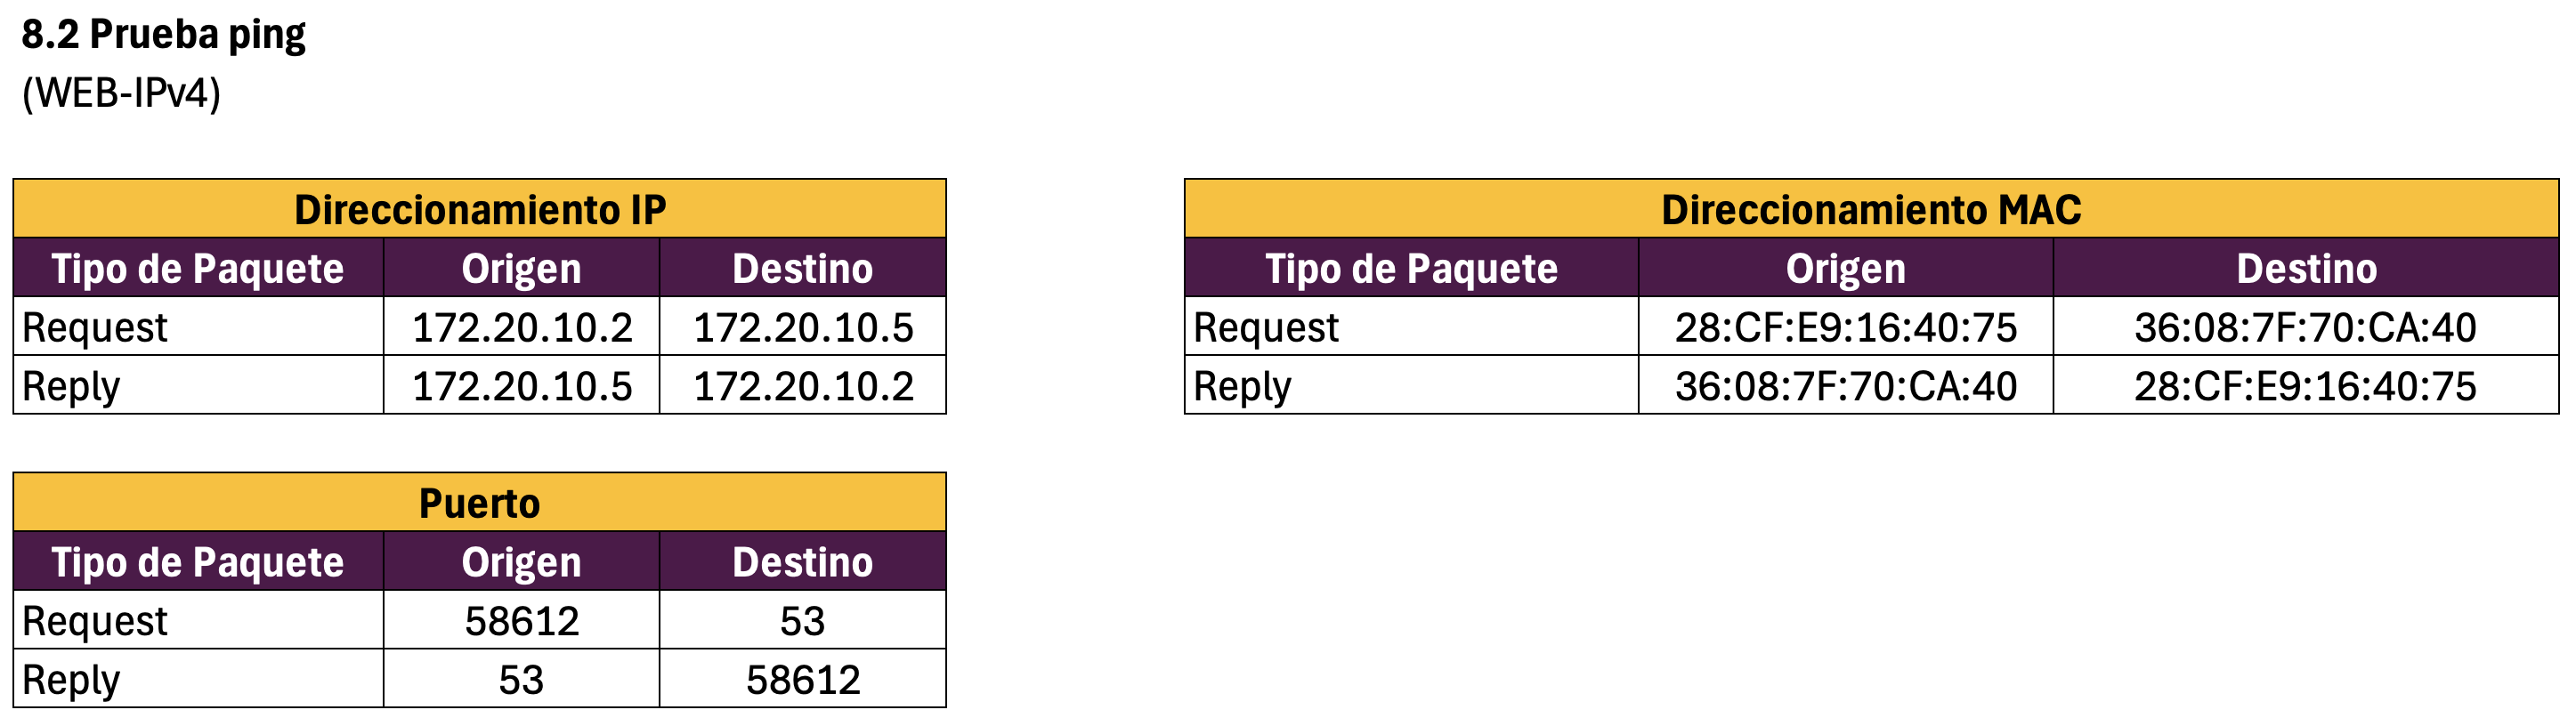
\includegraphics[width=0.85\textwidth]{lab-02-screenshots/8.2-WEB-IP-table}
    \caption{Tabla de IPs, MACs, y puertos origen/destino}
\end{figure}

%==============================================================
%=====================   8.3   ================================
%==============================================================
\renewcommand{\thesection}{8.\arabic{section}}
\section{Análisis de tráfico del Servicio FTP}

En esta sección se verifica el correcto funcionamiento del servicio FTP realizando una sesión autenticada desde el cliente para descargar y subir un archivo, capturando cada fase en los archivos \textcolor{blue}{\texttt{FTP\_download.pcap}} y \textcolor{blue}{\texttt{FTP\_upload.pcap}}. Usando Wireshark, se filtra el tráfico FTP para examinar los intercambios de control y de datos, y posteriormente se documentan los detalles de la capa de aplicación, el protocolo de transporte utilizado, y los puertos involucrados. 

\subsection{Conexión al servidor FTP}
El servidor responde primero con el mensaje de bienvenida. El cliente intenta establecer una sesión segura con AUTH TLS/SSL, pero el servidor lo rechaza con código \textcolor{red}{530} y solicita autenticación clásica (Esto se debe a que inicialmente configuré el servidor sde forma segura con vsfptd pero deshabilité la seguridad para poder observar bien el protocolo FTP). Luego el cliente envía \textcolor{red}{USER hermione} y \textcolor{red}{PASS test123}, a lo que el servidor responde con \textcolor{red}{230 Login successful}, confirmando el acceso. Luego, se ejecutan otros comandos donde el servido lista sus funcionalidades soportadas \textcolor{red}{(PASV, EPSV, MDTM, etc.)}. Todo este intercambio ocurre sobre TCP puerto 21 en el canal de control.


\begin{figure}[H]
    \centering
    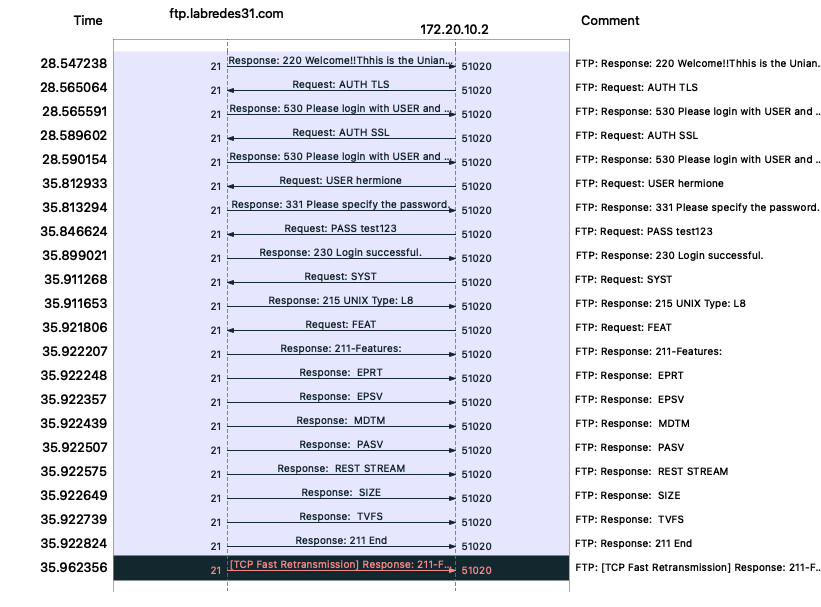
\includegraphics[width=0.85\textwidth]{lab-02-screenshots/8.3-FTP-start-session}
    \caption{Inicio de sesión FTP}
\end{figure}

\subsection{Descarga de archivo (Download)}
En esta parte se observa la navegación y transferencia de un archivo en FTP. Tras el mensaje \textcolor{red}{230 Login successful}, el cliente cambia al directorio \textcolor{red}{/files} con CWD y el servidor confirma con \textcolor{red}{250}. Luego el cliente consulta el directorio actua y solicita modo pasivo con 8.3-FTP-download-flow{PASV}. El servidor responde con la dirección y puerto a usar \textcolor{red}{(227 Entering Passive Mode)}. El cliente pide descargar el archivo \textcolor{red}{a.txt} con \textcolor{red}{RETR a.txt}, el servidor abre la conexión de datos \textcolor{red}{(150 Opening data connection)} y confirma la transferencia exitosa de este archivo con \textcolor{red}{226 Transfer complete.}

\begin{figure}[H]
    \centering
    \includegraphics[width=0.85\textwidth]{lab-02-screenshots/8.3-FTP-download-flow}
    \caption{Descarga de archivo por usuario "hermione"}
\end{figure}

\subsection{Carga de archivo (Upload)}
Después del inicio de sesión exitoso \textcolor{red}{(230 Login successful)}, el cliente cambia al directorio \textcolor{red}{/files} con \textcolor{red}{CWD /files}, confirmado por el servidor con \textcolor{red}{250 Directory successfully changed}. Luego verifica la ubicación con \textcolor{red}{PWD}, y el servidor responde con \textcolor{red}{257 "/files"}. El cliente ajusta el modo de transferencia a ASCII con TYPE A, y el servidor responde \textcolor{red}{200 Switching to ASCII mode}. Con el comando \textcolor{red}{PASV} se abre un canal de datos en modo pasivo, indicado por la respuesta \textcolor{red}{227 Entering Passive Mode}. Al final del proceso, el cliente solicita hacer upload del archivo \textcolor{red}{b.txt} con \textcolor{red}{STOR b.txt} y el servidor responde \textcolor{red}{150 Ok to send data} y, al finalizar la transferencia, confirma con \textcolor{red}{226 Transfer complete}.

En estas capturas no mostramos el hecho de que tenemos dos usuarios: "harry" y "hermione". Los archivos de "hermione" no son visibles desde POV del usuario de "harry"y vice versa. (Esto lo configuramos en \textcolor{blue}{/etc/vsftpd.conf})

\begin{figure}[H]
    \centering
    \includegraphics[width=0.85\textwidth]{lab-02-screenshots/8.3-FTP-upload-flow}
    \caption{Descarga de archivo por usuario "hermione"}
\end{figure}
%==============================================================
%=====================   8.4   ================================
%==============================================================
\renewcommand{\thesection}{8.\arabic{section}}
\section{Análisis de tráfico del Servicio Web}
En esta sección se analiza el funcionamiento del protocolo HTTP dentro de la topología configurada. Mediante capturas en Wireshark, se observan las peticiones y respuestas entre el cliente y el servidor web en texto claro, lo que permite identificar directamente los encabezados y contenidos intercambiados, así como los puertos y el protocolo de transporte utilizados en la comunicación. El tráfico generado se capturó y se guardó en el archivo \textcolor{blue}{\texttt{Ping\_WEB\_view.pcap}}
\subsection{Acceso al servidor web mediante HTTP}
En esta captura se observa primero la resolución DNS de \textcolor{blue}{web.labredes31.com}. A continuación, el cliente establece una conexión TCP con el servidor en el puerto 80, completando el three-way handshake. Luego, el cliente envía una petición \textcolor{red}{GET / HTTP/1.1} y el servidor responde con \textcolor{red}{HTTP/1.1 200 OK}, entregando la página en plaintext. Luego el cliente solicita el recurso \textcolor{red}{/favicon.ico}, que también recibe una respuesta satisfactoria \textcolor{red}{200 OK}. Finalmente, la comunicación se cierra correctamente mediante el intercambio de mensajes \textcolor{red}{FIN, ACK}, completando así el ciclo típico de una sesión HTTP.


\begin{figure}[H]
    \centering
    \includegraphics[width=0.85\textwidth]{lab-02-screenshots/8.4-HTTP-flow}
    \caption{Flow de HTTP}
\end{figure}


\begin{figure}[H]
    \centering
    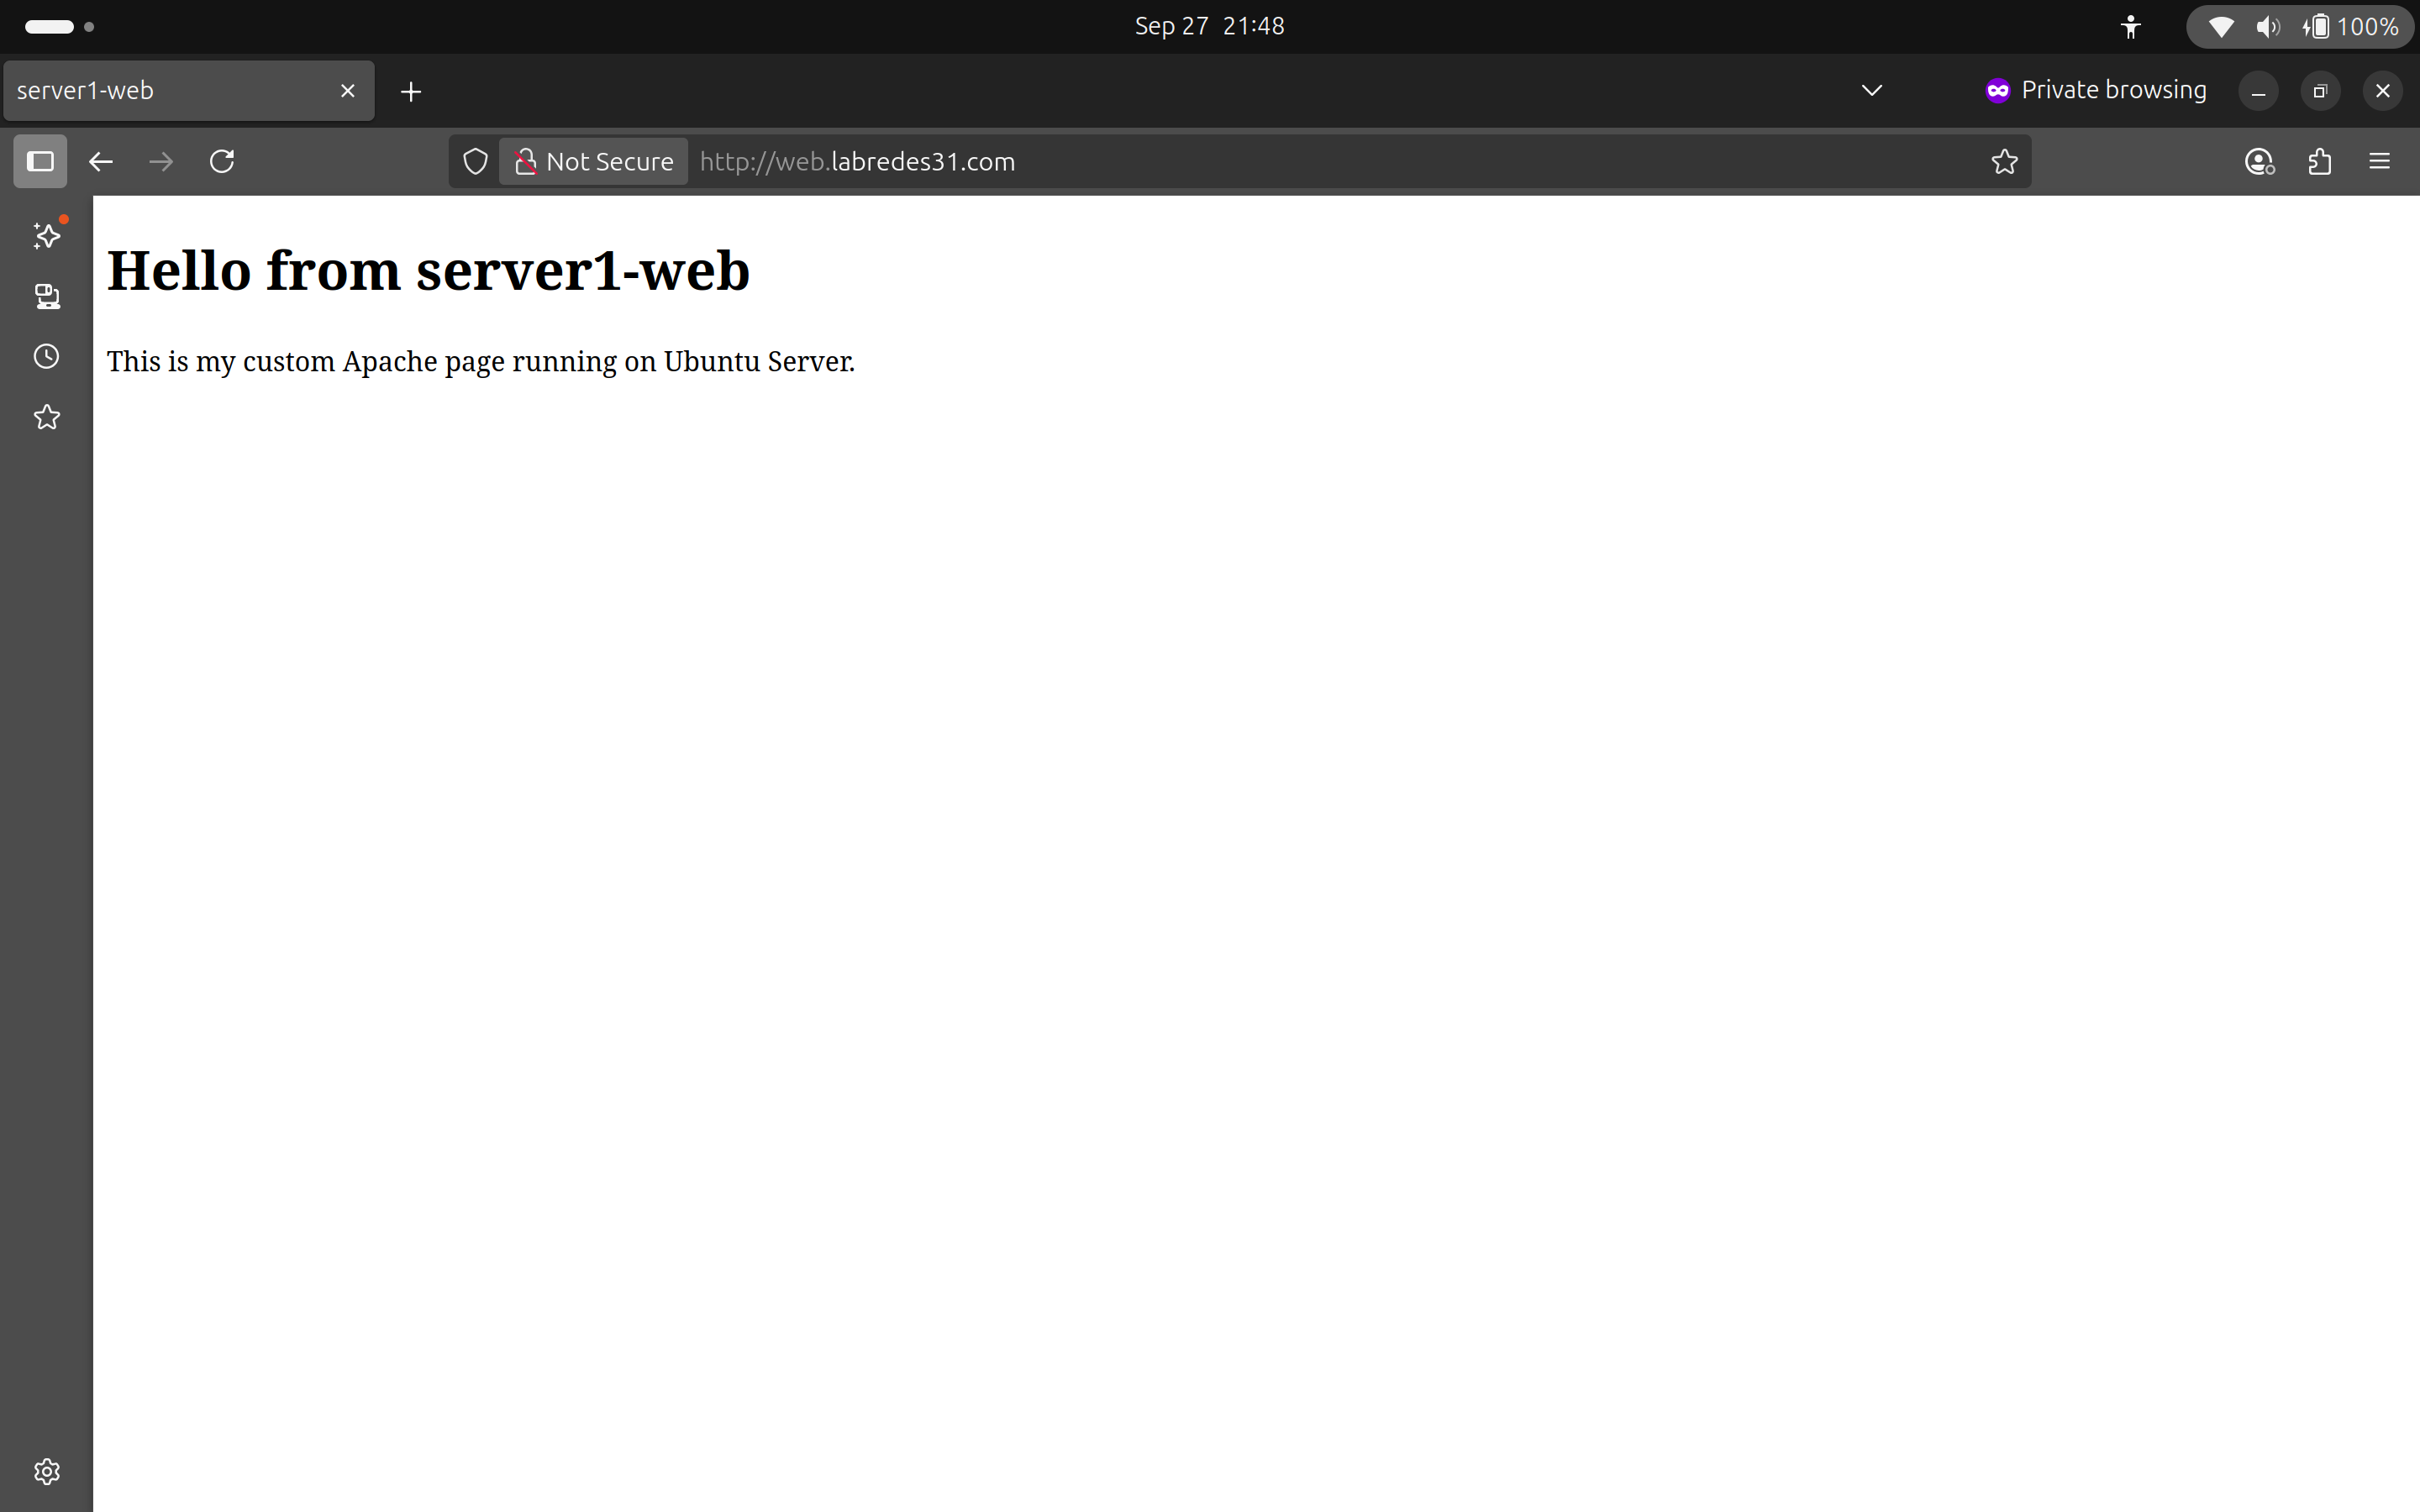
\includegraphics[width=0.85\textwidth]{lab-02-screenshots/8.4-web-browser}
    \caption{Vista de página web desde buscador en Ubuntu Client}
\end{figure}


%==============================================================
%=====================   8.5   ================================
%==============================================================
\renewcommand{\thesection}{8.\arabic{section}}
\section{Análisis del protocolo HTTPS realizando navegación en el sitio de YouTube}

\subsection{Navegación en YouTube}
Se realizó la captura de tráfico mientras se navegaba en \textbf{https://www.youtube.com/}. 
Para reducir interferencias, se mantuvo una única pestaña activa en el navegador; se inició sesión con cuenta de Google y se realizaron acciones de navegación/comentarios. 
La captura se guardó como \texttt{YouTube\_view.pcapng}.

\begin{itemize}
    \item \textbf{Filtro aplicado en Wireshark:} \texttt{tcp.port == 443}.
    \item \textbf{Capa de aplicación (TLS):} Se observan mensajes del \textit{handshake TLS} (\textit{Client Hello}, \textit{Server Hello}, \textit{Certificate}) y posteriormente \textit{Application Data}, que corresponde a tráfico HTTP cifrado.
    \item \textbf{Capa de transporte (TCP):} HTTPS se ejecuta sobre TCP, lo que provee fiabilidad mediante control de flujo, numeración de secuencia y \textit{ACKs}.
    \item \textbf{Puertos:} Destino \textbf{443} (HTTPS) y puertos de origen efímeros.
    \item \textbf{SNI/servidores:} \texttt{youtube.com}, \texttt{accounts.youtube.com} y dominios relacionados.
\end{itemize}

\noindent\textbf{Conclusión (YouTube):} 
El tráfico está protegido mediante TLS (1.2/1.3). 
El contenido de peticiones/respuestas HTTP no es visible (aparece como \textit{Application Data}), garantizando confidencialidad e integridad.

%--------------------------------------------------------------
\subsection{Navegación en otros sitios HTTPS}
Se realizó una segunda captura visitando: \textbf{www.elespectador.com}, \textbf{www.eltiempo.com}, \textbf{www.uniandes.edu.co} y \textbf{www.bancolombia.com} (\texttt{HTTPS\_view.pcapng}). 
En todos los casos se evidenció \textbf{TLS} sobre \textbf{TCP/443}, con presencia de \textit{Client Hello}/\textit{Server Hello}/\textit{Application Data}.

\noindent\textbf{Conclusión (otros sitios):}
Todos emplean HTTPS; se identificaron versiones TLS 1.2/1.3 según el host. 
El cifrado impide visualizar el contenido HTTP en claro.

%==============================================================
%=====================   Flujos   =============================
%==============================================================
\subsection*{Representación gráfica de flujos}

\begin{figure}[H]
    \centering
    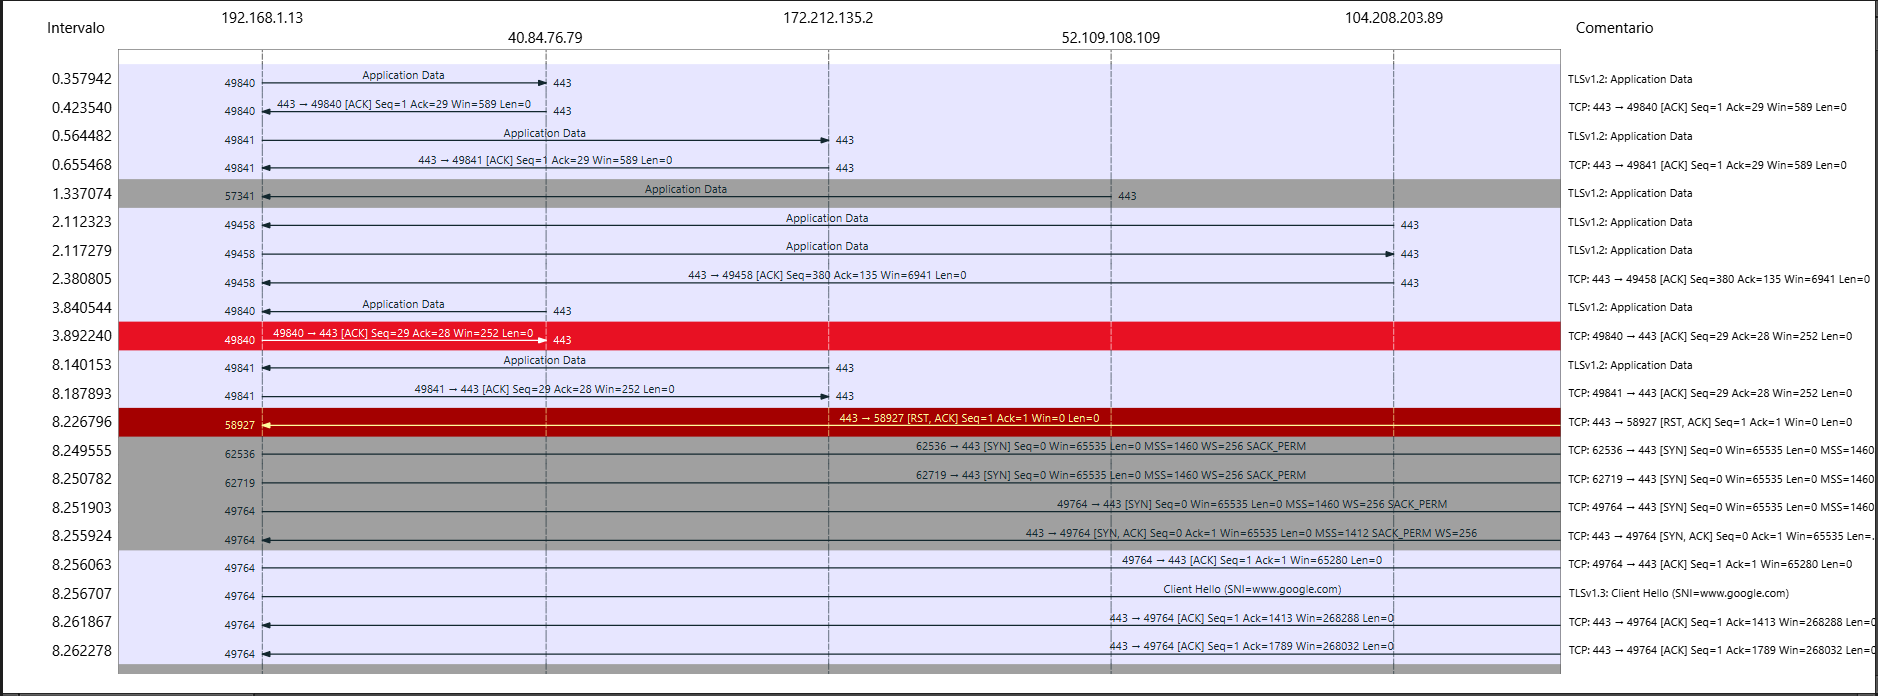
\includegraphics[width=0.95\textwidth]{lab-02-screenshots/8.5-YouTube-flow.png}
    \caption{Flujo de comunicación durante la navegación en YouTube. Se aprecian múltiples \texttt{Application Data} (tráfico cifrado) y \texttt{ACKs} propios de TCP hacia distintos hosts de Google/YouTube.}
\end{figure}

\begin{figure}[H]
    \centering
    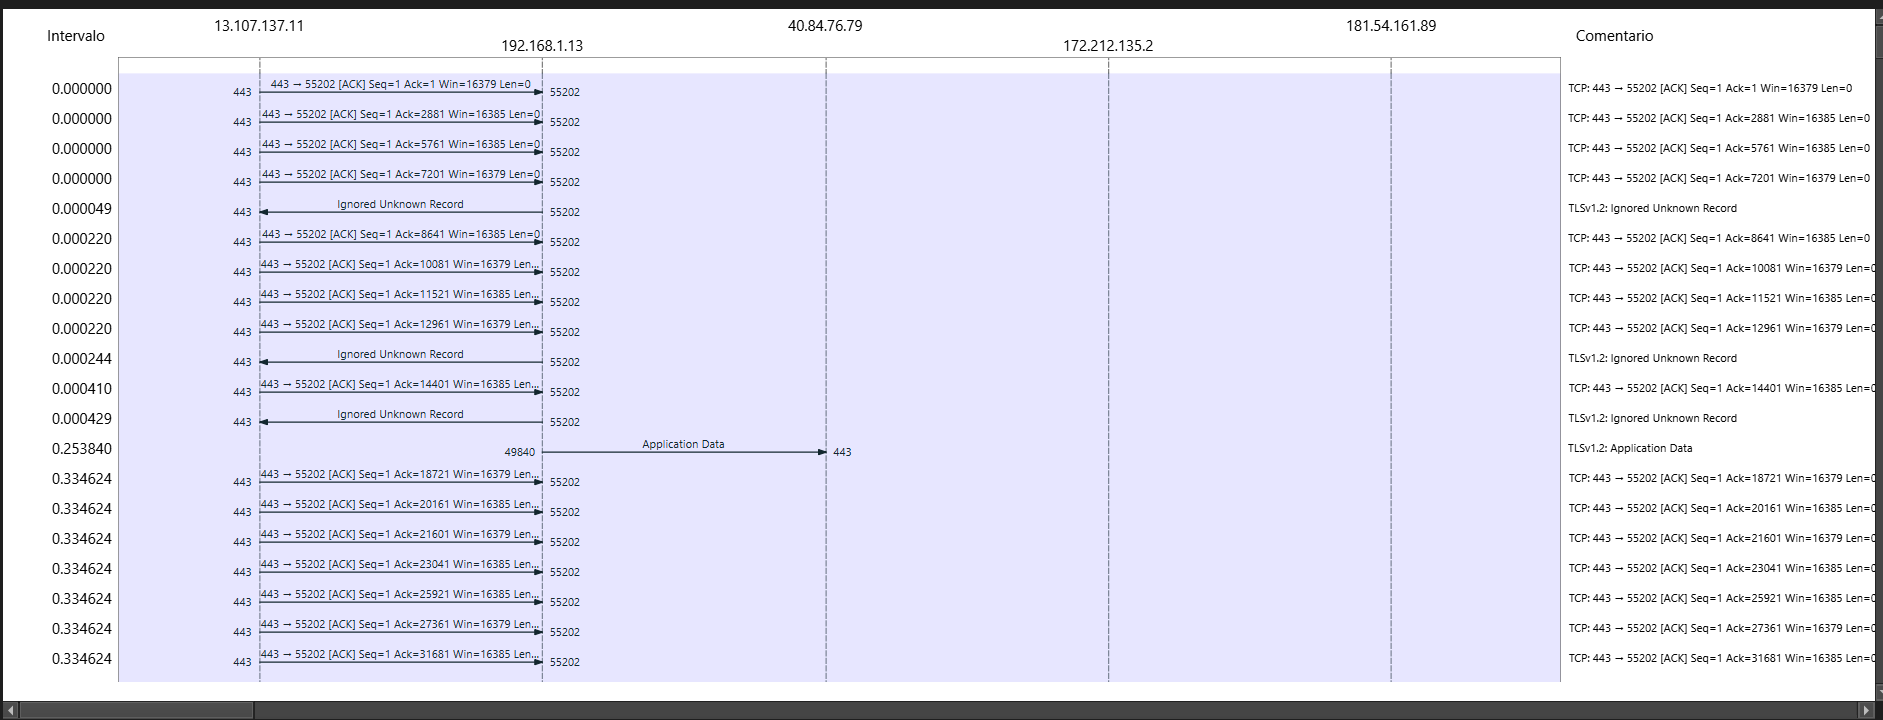
\includegraphics[width=0.95\textwidth]{lab-02-screenshots/8.5-HTTPS-flow.png}
    \caption{Flujo durante la navegación en sitios HTTPS (El Espectador, El Tiempo, Uniandes y Bancolombia). Se observa el establecimiento de conexión (SYN/SYN-ACK/ACK) y el posterior \textit{handshake TLS} (por ejemplo, \textit{Client Hello}).}
\end{figure}

%==============================================================
%=================== Evidencia de Capas =======================
%==============================================================
\subsection*{Análisis de la Capa de Aplicación (TLS)}

Durante el \textit{handshake TLS}, el cliente envía un \texttt{Client Hello} indicando versiones soportadas (TLS 1.2/1.3), \textit{cipher suites} y el nombre del servidor (\textit{SNI}). 
El servidor responde con \texttt{Server Hello} seleccionando parámetros criptográficos y entrega su \textit{Certificate} (X.509) para autenticación. 
Tras la negociación de claves, la sesión opera con \texttt{Application Data} (HTTP cifrado).

\begin{figure}[H]
    \centering
    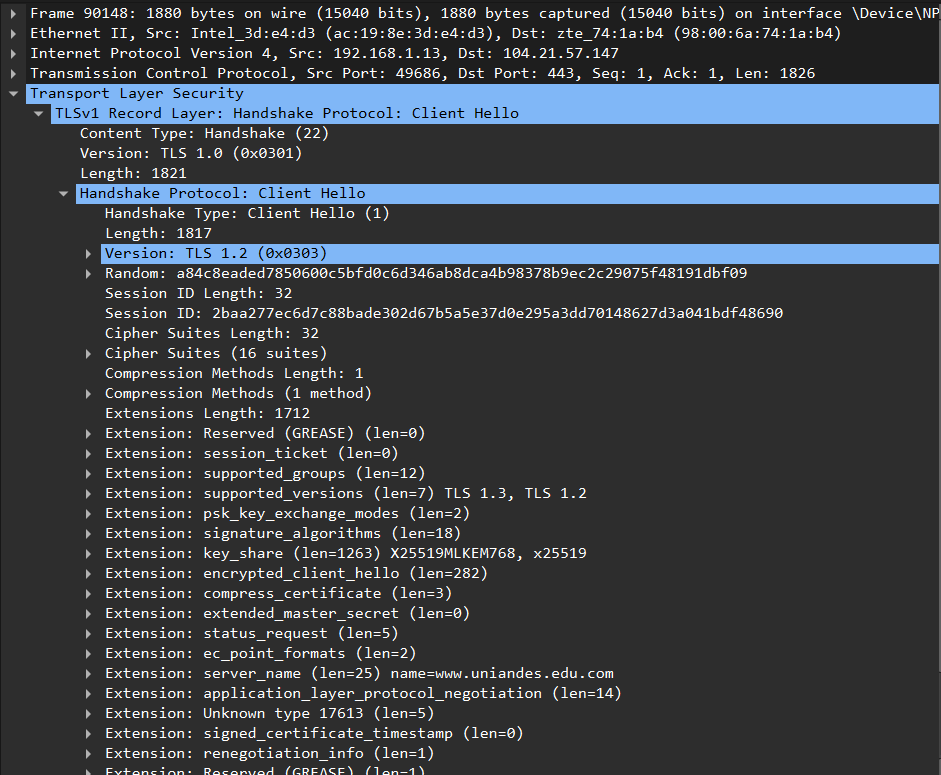
\includegraphics[width=0.9\textwidth]{lab-02-screenshots/8.5-CapaAplicacion-HTTPS.png}
    \caption{\texttt{Client Hello} hacia \texttt{www.uniandes.edu.co}. Se observan extensiones TLS (p.\,ej., \textit{supported\_versions}, \textit{server\_name}).}
\end{figure}

\begin{figure}[H]
    \centering
    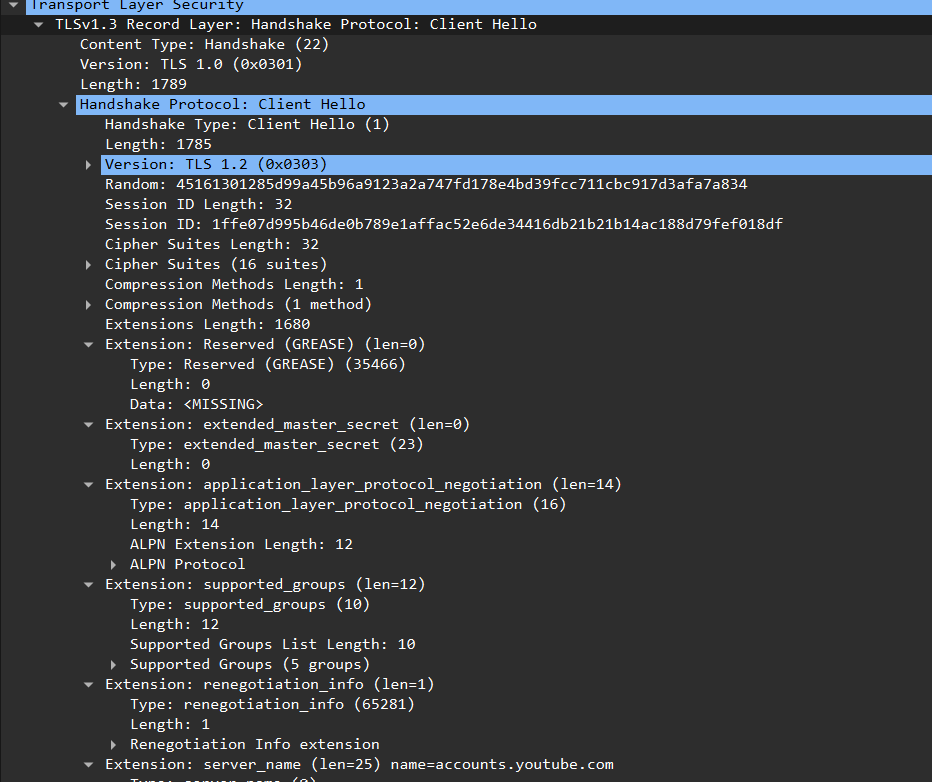
\includegraphics[width=0.9\textwidth]{lab-02-screenshots/8.5-CapaAplicacion-Youtube.png}
    \caption{\texttt{Client Hello} hacia \texttt{accounts.youtube.com}. Se evidencia el uso de TLS 1.2/1.3, \textit{cipher suites} ofrecidas y el SNI del host.}
\end{figure}

\noindent\textit{Implicación:} la capa de aplicación expone la negociación TLS, pero el contenido HTTP queda cifrado.

%--------------------------------------------------------------
\subsection*{Análisis de la Capa de Transporte (TCP)}

HTTPS requiere de TCP para asegurar fiabilidad (entrega ordenada, control de congestión) y se inicia con el \textit{three-way handshake} (SYN, SYN-ACK, ACK). 
En las capturas se aprecian campos como puertos origen/destino, números de secuencia, ventana y flags (\texttt{PSH}, \texttt{ACK}), además del \textit{payload} que TLS cifra.

\begin{figure}[H]
    \centering
    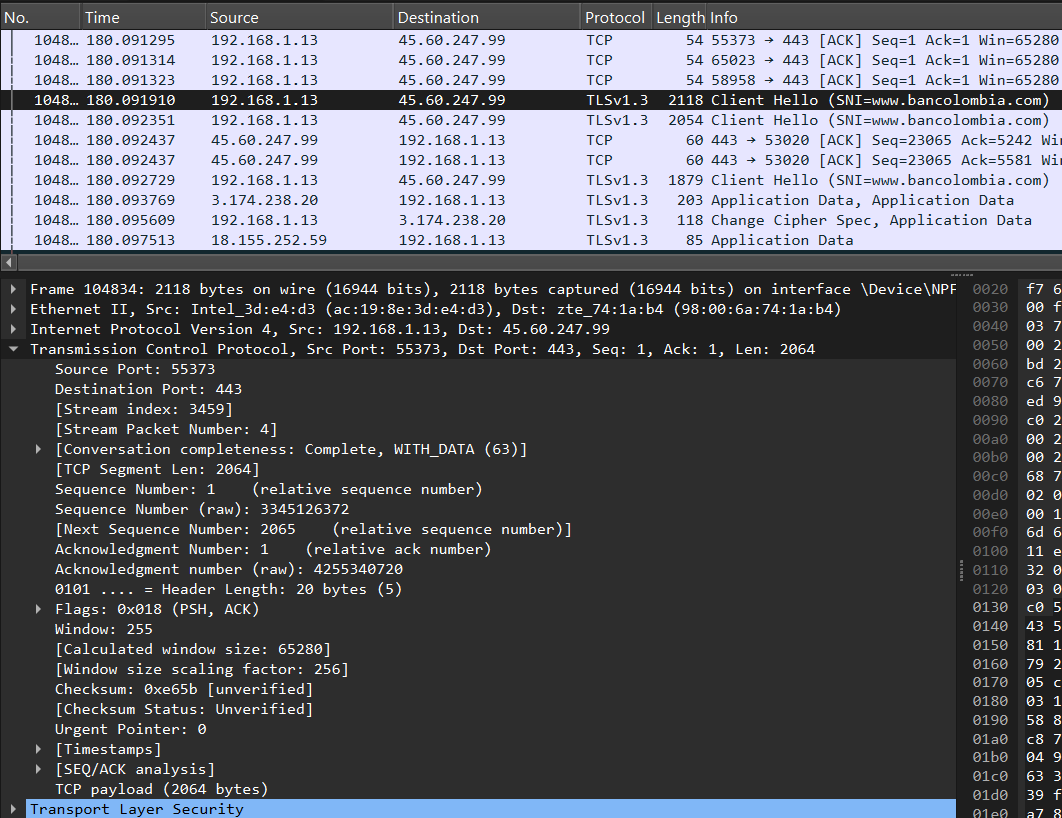
\includegraphics[width=0.9\textwidth]{lab-02-screenshots/8.5-CapaTransporte-HTTPS.png}
    \caption{Detalle TCP hacia \texttt{www.bancolombia.com}: puertos, números de secuencia/ack, ventana y \texttt{TCP payload} (transportado por TLS).}
\end{figure}

\begin{figure}[H]
    \centering
    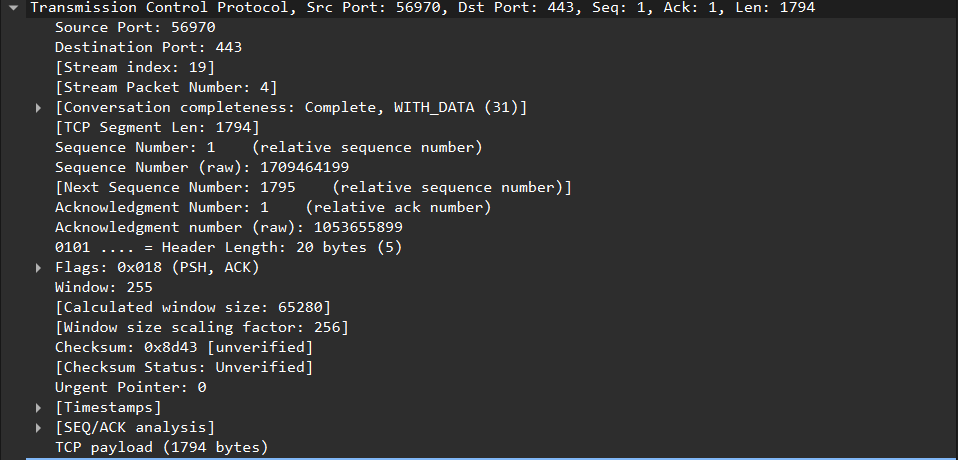
\includegraphics[width=0.9\textwidth]{lab-02-screenshots/8.5-CapaTransporte-Youtube.png}
    \caption{Paquete TCP en conexión a YouTube mostrando longitud de segmento, flags y \texttt{TCP payload}; el contenido de aplicación va cifrado por TLS.}
\end{figure}

%==============================================================
%=================== Evidencia por Sitio ======================
%==============================================================
\subsection*{Evidencia de paquetes HTTPS por sitio web}

\begin{figure}[H]
    \centering
    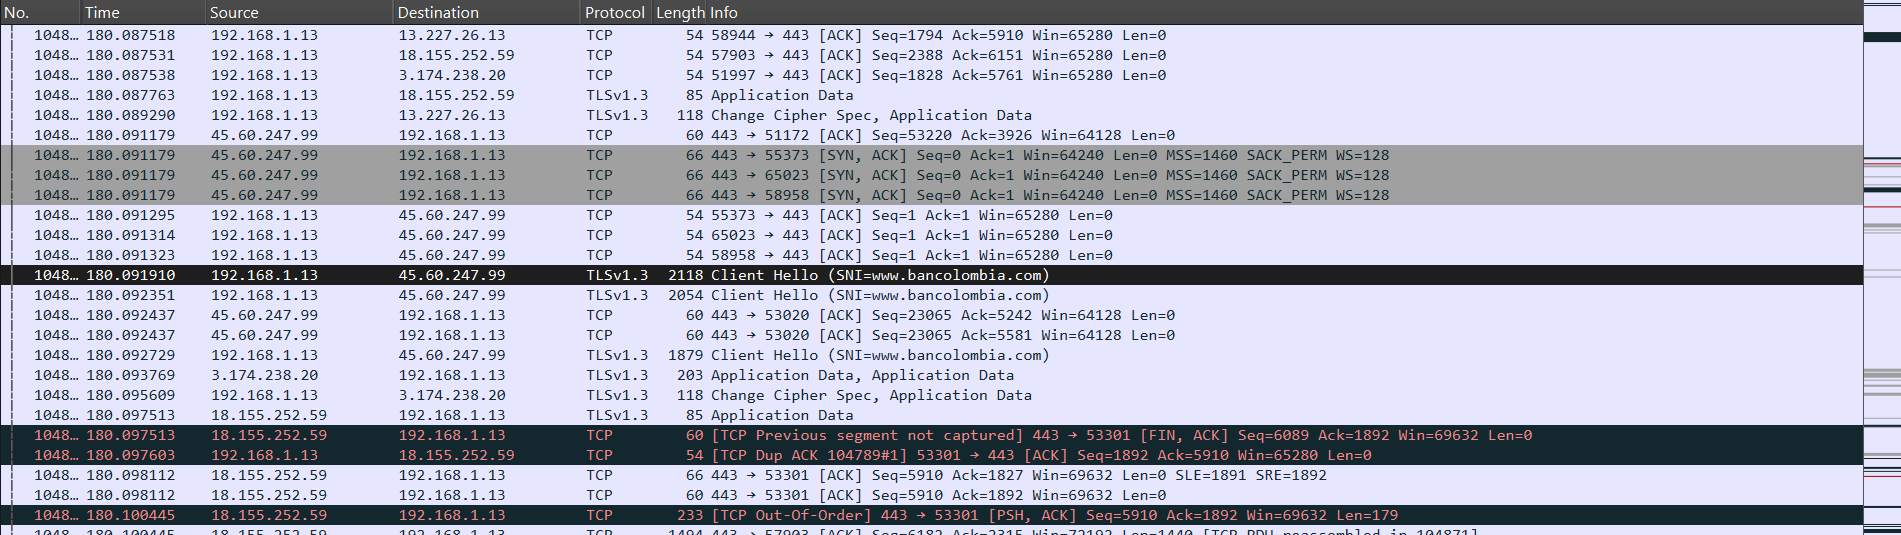
\includegraphics[width=0.95\textwidth]{lab-02-screenshots/8.5-HTTPS-bancolombia.png}
    \caption{\texttt{Client Hello} hacia \texttt{www.bancolombia.com} (TLS 1.3). Evidencia del inicio del \textit{handshake} y establecimiento de un canal cifrado adecuado para datos financieros.}
\end{figure}

\begin{figure}[H]
    \centering
    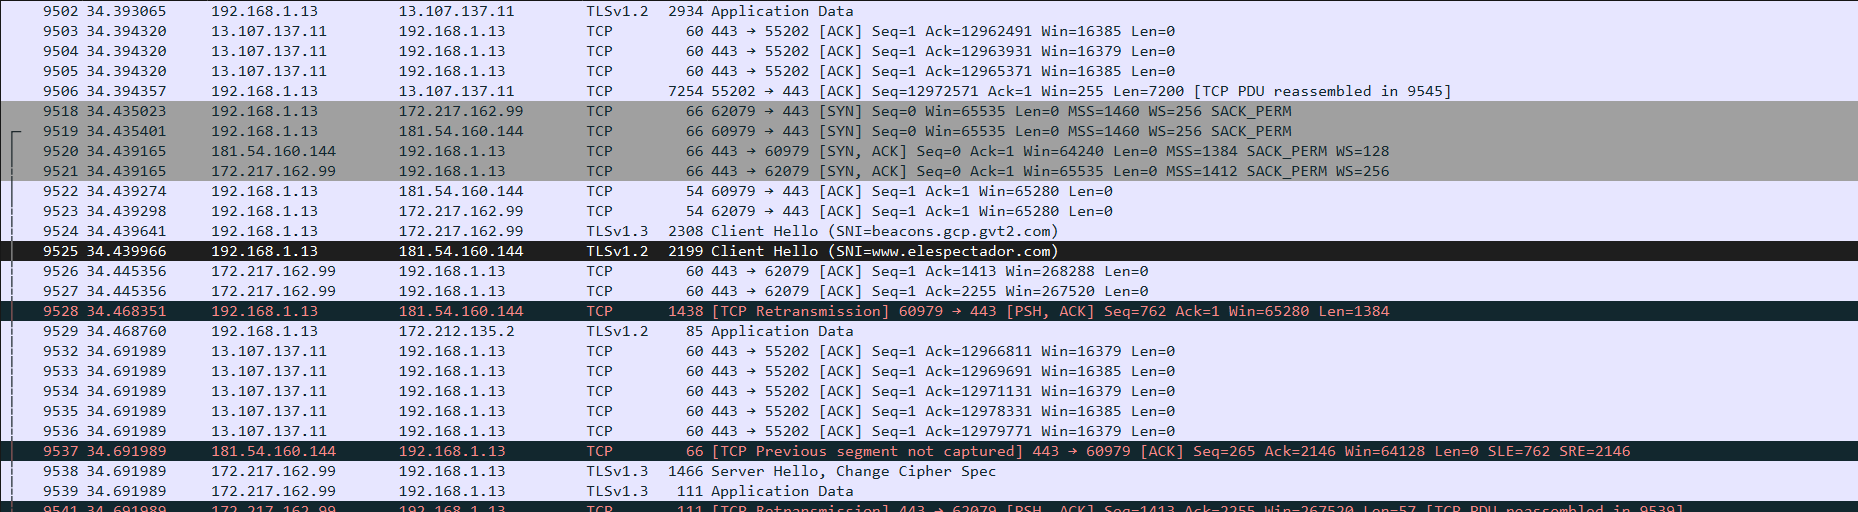
\includegraphics[width=0.95\textwidth]{lab-02-screenshots/8.5-HTTPS-elespectador.png}
    \caption{Conexión a \texttt{www.elespectador.com}. Se visualiza \texttt{Client Hello} (TLS 1.2) y, a continuación, \texttt{Application Data} (HTTP sobre TLS).}
\end{figure}

\begin{figure}[H]
    \centering
    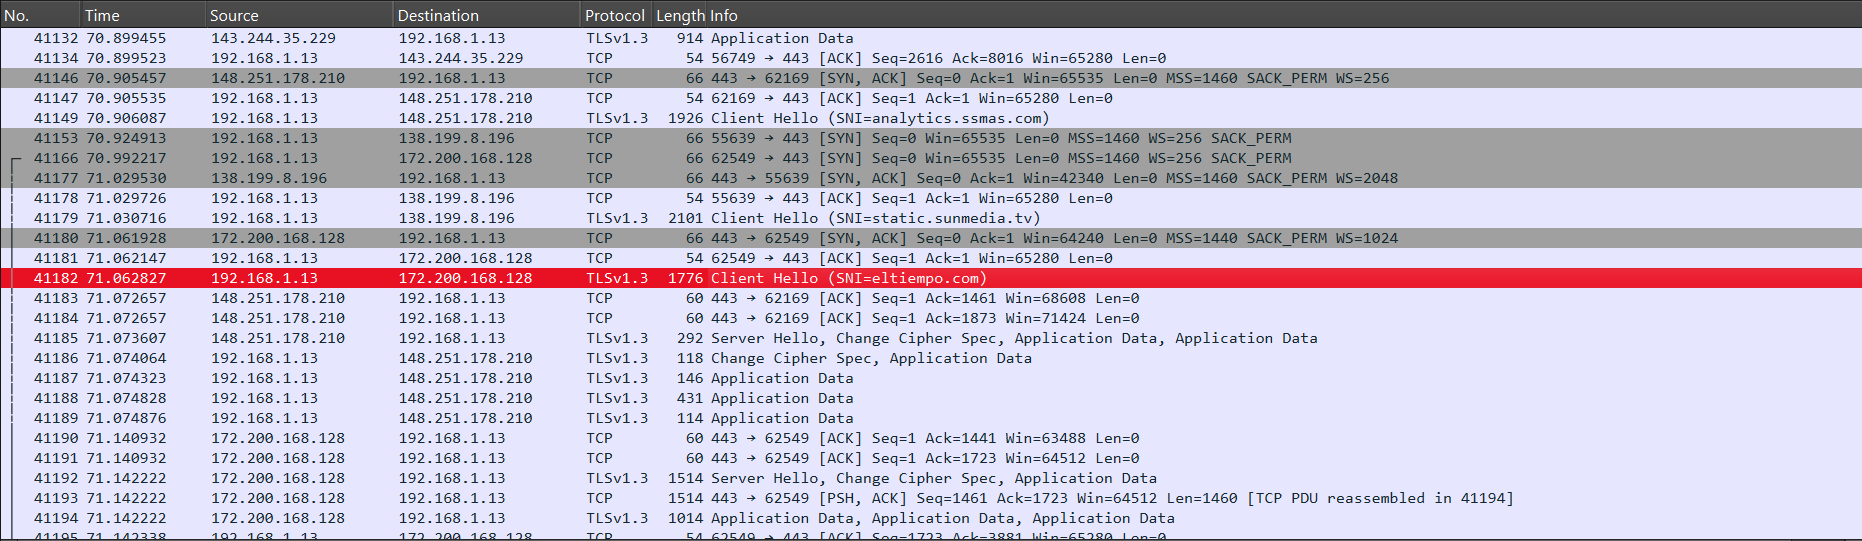
\includegraphics[width=0.95\textwidth]{lab-02-screenshots/8.5-HTTPS-eltiempo.png}
    \caption{Tráfico hacia \texttt{www.eltiempo.com}: \texttt{Client Hello} en TLS 1.3 seguido de \texttt{Server Hello}/\texttt{Change Cipher Spec} y \texttt{Application Data}.}
\end{figure}

\begin{figure}[H]
    \centering
    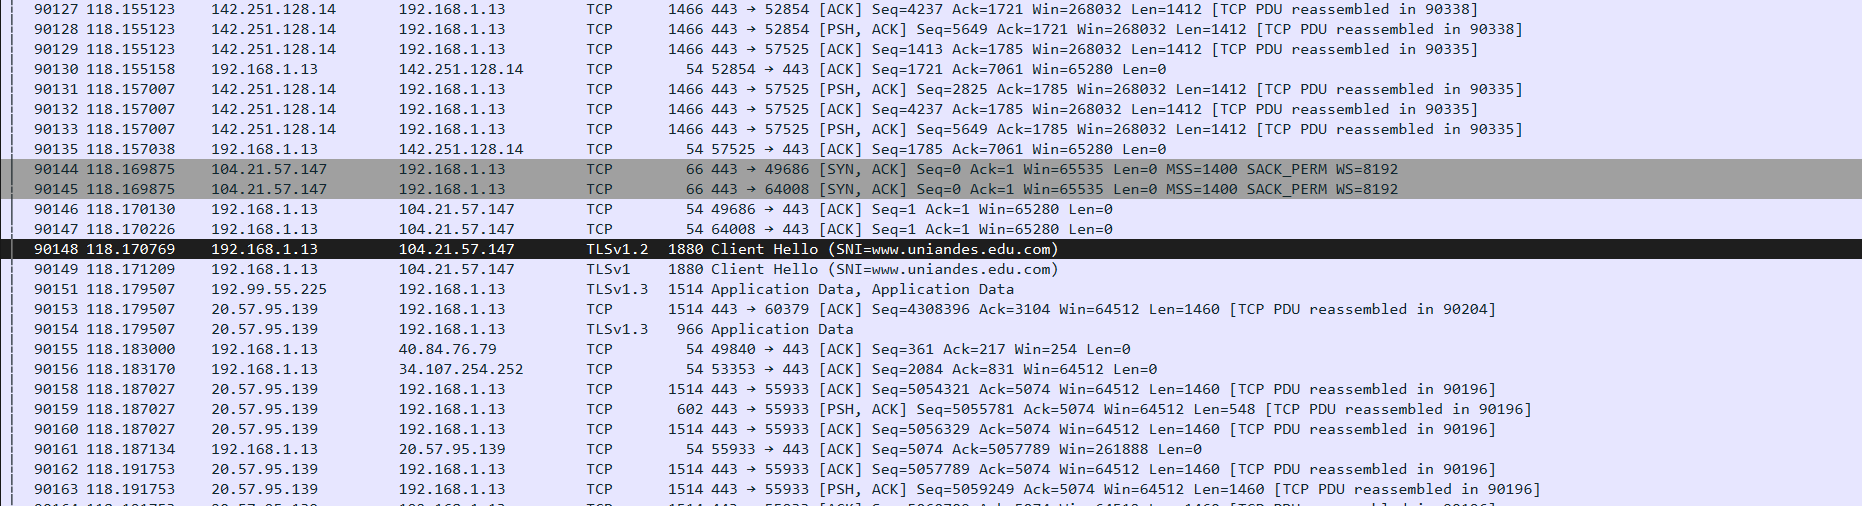
\includegraphics[width=0.95\textwidth]{lab-02-screenshots/8.5-HTTPS-uniandes.png}
    \caption{Tráfico hacia \texttt{www.uniandes.edu.co}. Evidencia de \texttt{Client Hello} con SNI del host y negociación de versiones/cifrados.}
\end{figure}

%--------------------------------------------------------------
\subsection*{Evidencia de paquetes en YouTube}

\begin{figure}[H]
    \centering
    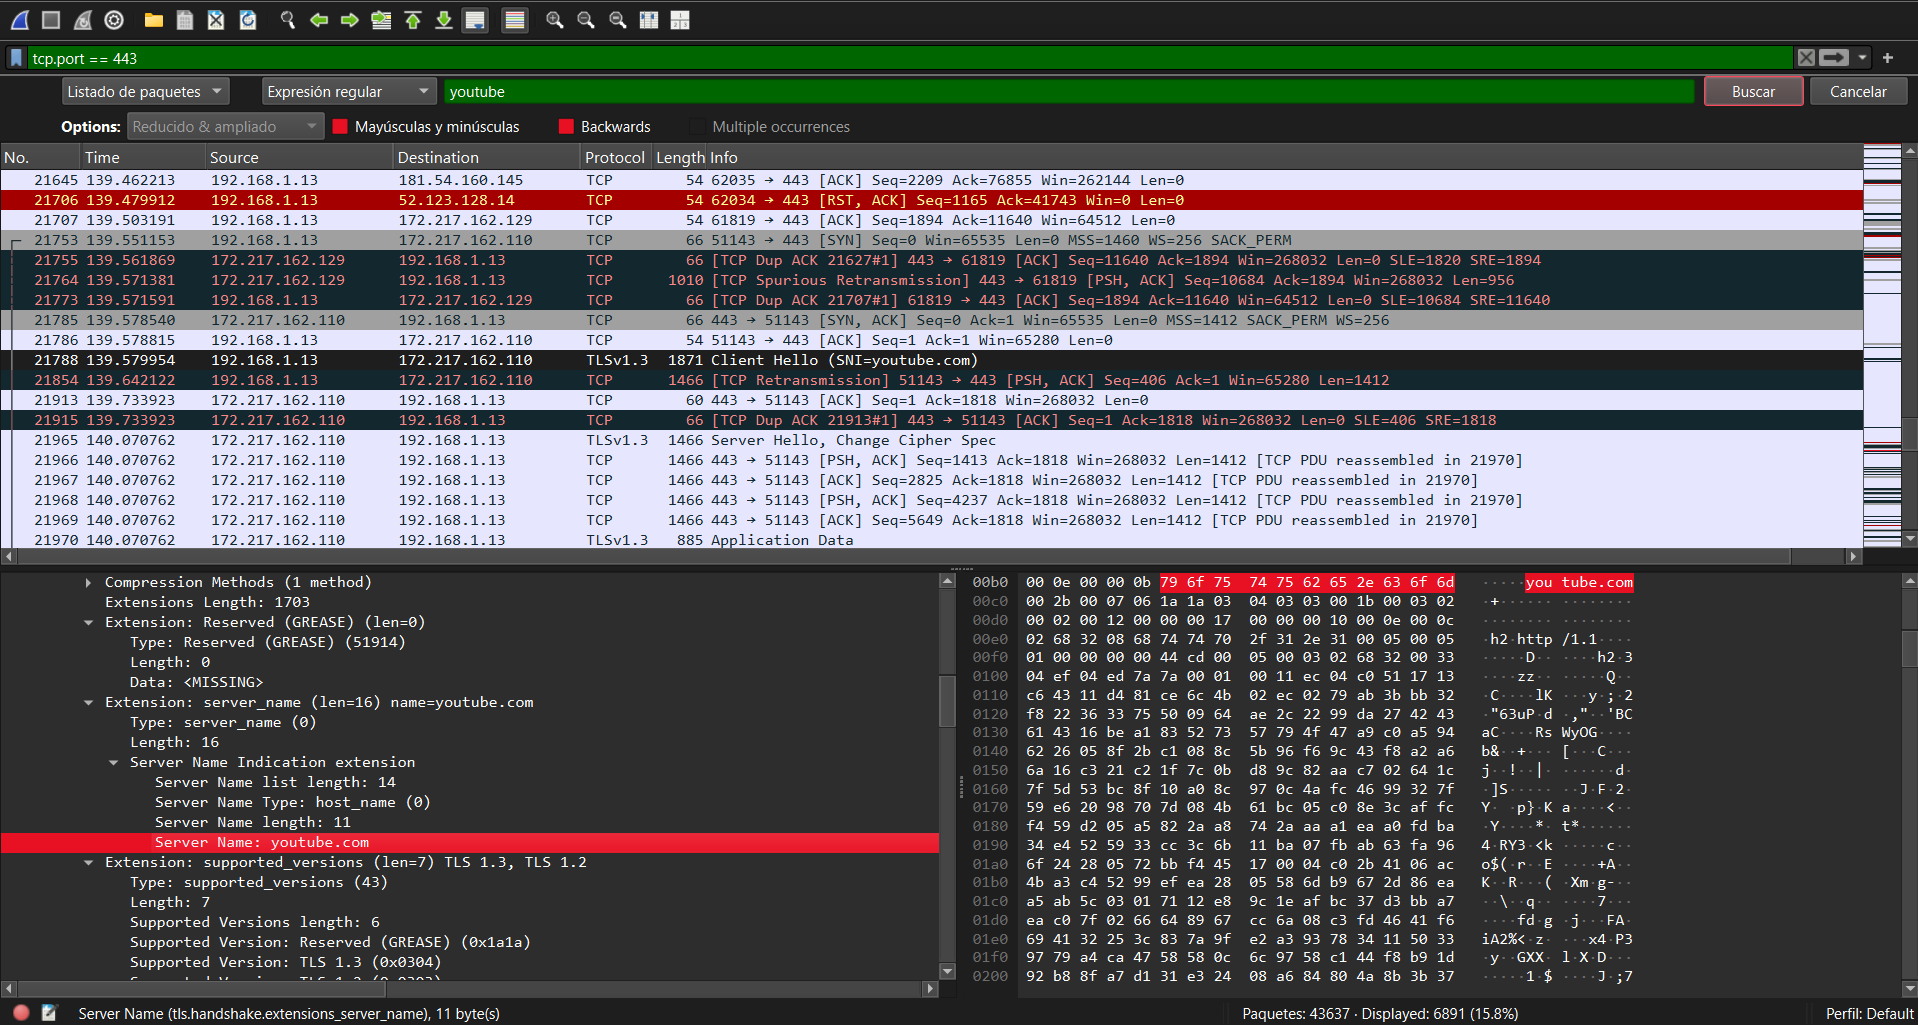
\includegraphics[width=0.95\textwidth]{lab-02-screenshots/8.5-Packets-Youtube.png}
    \caption{Listado filtrado por \texttt{tcp.port == 443} con conexiones a \texttt{youtube.com}. Se observan \textit{handshake TLS} y posteriormente \texttt{Application Data}.}
\end{figure}

\begin{figure}[H]
    \centering
    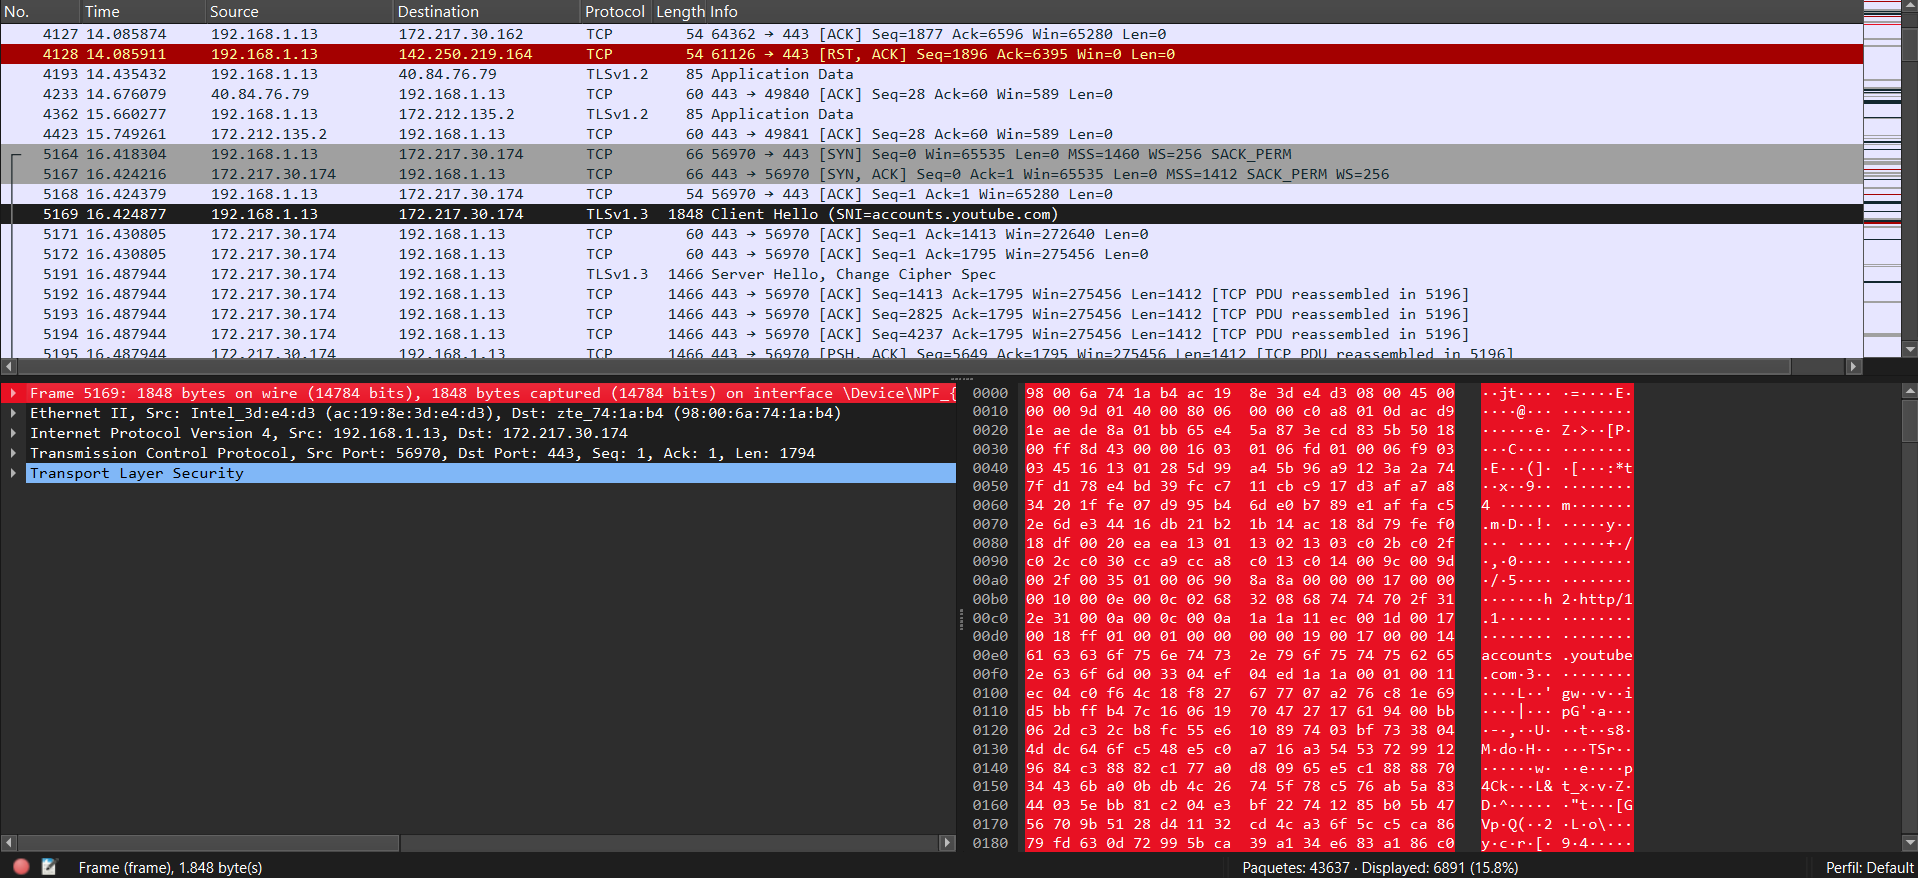
\includegraphics[width=0.95\textwidth]{lab-02-screenshots/8.5-Paquete-Youtube.png}
    \caption{Detalle de un paquete TLS asociado a YouTube: la capa de aplicación aparece como \texttt{Application Data}, confirmando el cifrado del contenido HTTP.}
\end{figure}

%==============================================================
%======================= Tablas (opc) =========================
%==============================================================
\subsection*{Ejemplos de paquetes (tabla)}
% Requiere \usepackage{array} si deseas columnas con p{..}
\begin{table}[H]
\centering
\caption{Ejemplos representativos de paquetes capturados (YouTube)}
\begin{tabular}{|c|c|c|c|c|}
\hline
\textbf{Fuente} & \textbf{Destino} & \textbf{Protocolo} & \textbf{Puerto Origen} & \textbf{Puerto Destino} \\
\hline
192.168.1.13 & \textit{YouTube/Google IP} & TCP (TLS 1.3) & \textit{efímero} & 443 \\
192.168.1.13 & \textit{YouTube/Google IP} & TCP (TLS 1.2) & \textit{efímero} & 443 \\
\hline
\end{tabular}
\end{table}

\begin{table}[H]
\centering
\caption{Ejemplos representativos de paquetes (otros sitios HTTPS)}
\begin{tabular}{|c|c|c|c|c|}
\hline
\textbf{Fuente} & \textbf{Destino} & \textbf{Protocolo} & \textbf{Puerto Origen} & \textbf{Puerto Destino} \\
\hline
192.168.1.13 & \textit{bancolombia.com (IP)} & TCP (TLS 1.3) & \textit{efímero} & 443 \\
192.168.1.13 & \textit{uniandes.edu.co (IP)} & TCP (TLS 1.2/1.3) & \textit{efímero} & 443 \\
\hline
\end{tabular}
\end{table}

%==============================================================
%==================== Cierre/Análisis =========================
%==============================================================
\subsection*{Conclusiones generales}
\begin{itemize}
    \item HTTPS combina HTTP con TLS sobre TCP/443, garantizando \textbf{confidencialidad}, \textbf{integridad} y \textbf{autenticación} del servidor mediante certificados X.509.
    \item Las capturas muestran el \textbf{handshake TLS} (\texttt{Client Hello}, \texttt{Server Hello}, \texttt{Certificate}) seguido de \texttt{Application Data} (HTTP cifrado), por lo cual el contenido de aplicación no es legible.
    \item El uso de TCP evidencia control de fiabilidad (SYN/SYN-ACK/ACK, números de secuencia, ventanas y \texttt{ACKs}).
    \item En YouTube se observan múltiples flujos cifrados (\texttt{Application Data}) por la naturaleza de \textit{streaming} y recursos; en los demás sitios se confirma el mismo patrón de seguridad.
\end{itemize}



%==============================================================
%=====================   8.6  ================================
%==============================================================
\renewcommand{\thesection}{8.\arabic{section}}
\section{Análisis del protocolo VoIP}
\subsection{Establecimiento de la llamada}

Empezaremos describiendo como se establece la conexion entre el servidor y aquellos clientes que se conectan para establecer las llamadas. Para esto, se hace uso del protocolo de capa de aplicacion SIP (Session Initiation Protocol) por el cual utilizara codigos de estados, (muy parecido a como funciona en HTTP) para indicar si el cliente se le permite establecer conexion para poder realizar las llamadas. A continuacion podremos ver como funciona este proceso:

\begin{figure}[H]
    \centering
    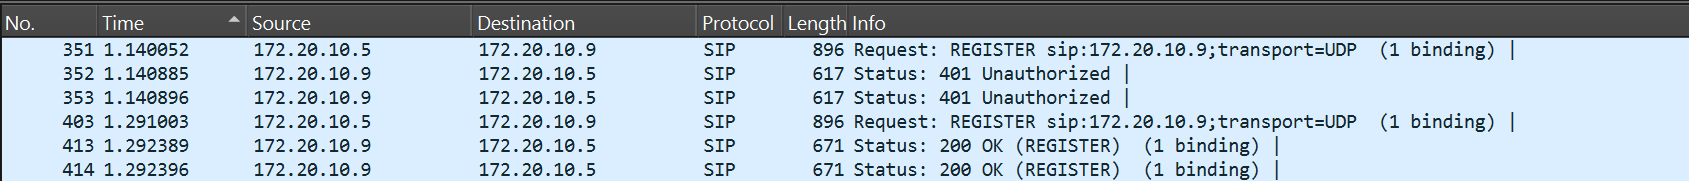
\includegraphics[width=0.95\textwidth]{lab-02-screenshots/8.6-inicioLlamada.png}
    \caption{Proceso de registro usando el protocolo SIP.}
\end{figure}

Aqui podemos ver como incialmente el cliente envia un request \textit{REGISTER} cuya respuesta es conexion con el servidor con el codigo de estatus \textit{401 Unauthorized}, esto porque introducimos una contraseña incorrecta; despues de esto se vuelve a intentar el registro del cliente, seguido por una respuesta de codigo de estado \textit{200 OK (REGISTER)}.
\subsection*{Uso de la capa de aplicacion}
Para el caso de las llamadas de aplicacion usadas por VoIP, solo tenemos el protocolo \textbf{SIP} utilizado para el registro de los clientes, su autorizacion y el manejo de sesion. A continuacion veremos mas a detalle el contenido de estos paquetes y los encabezados que utiliza.

\begin{figure}[H]
    \centering
    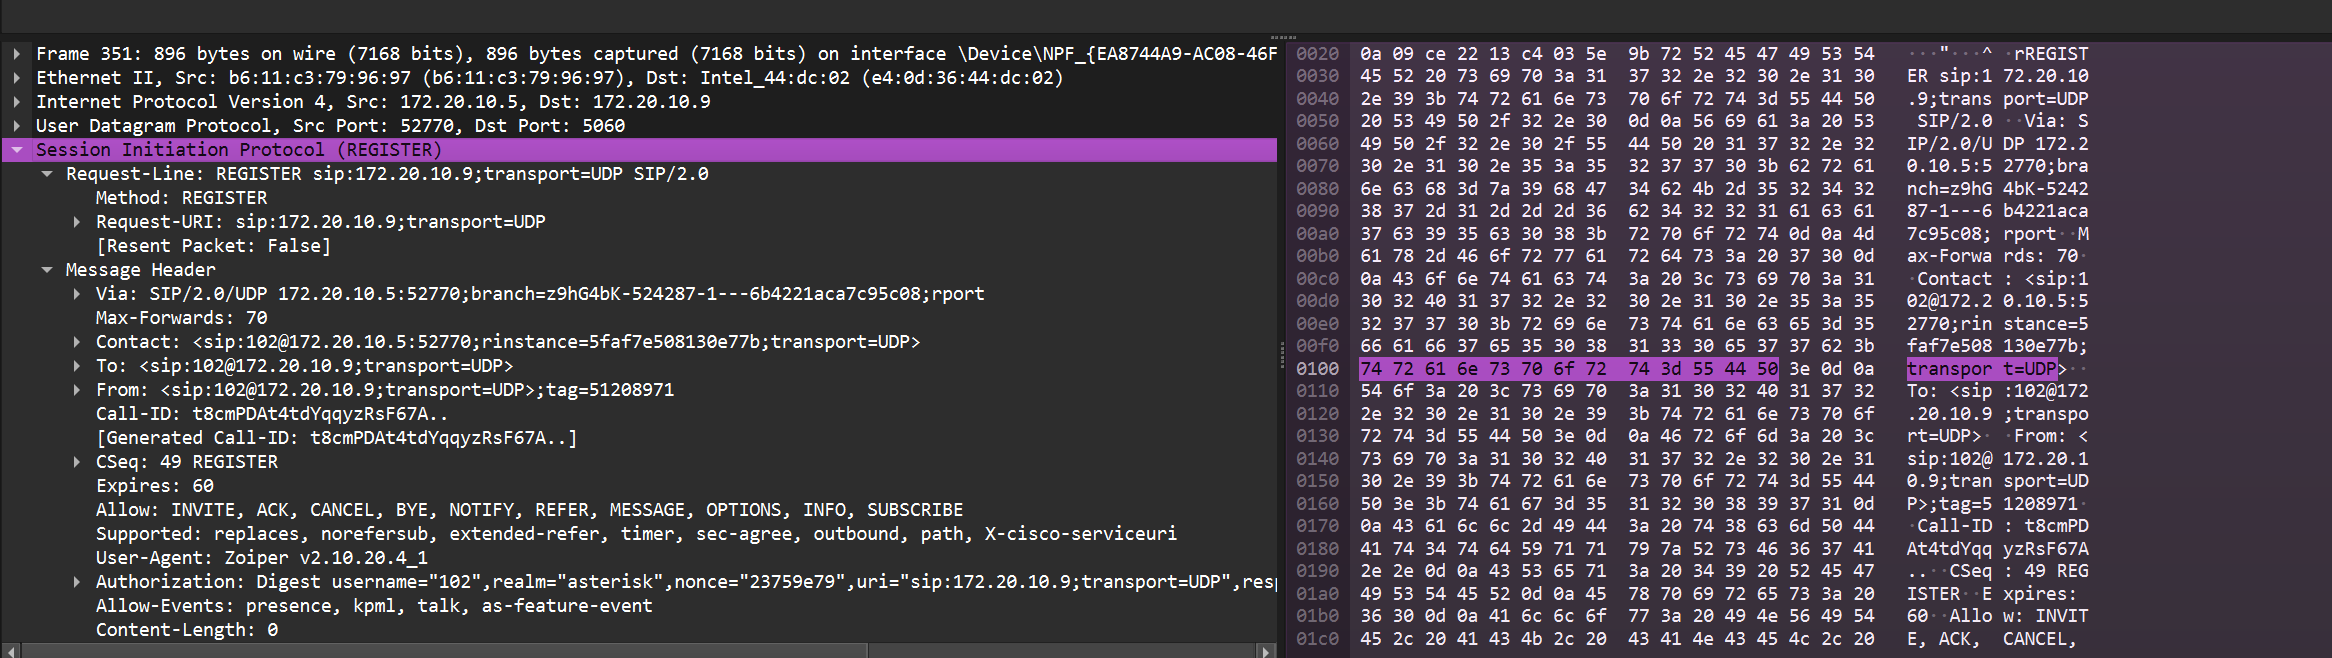
\includegraphics[width=0.95\textwidth]{lab-02-screenshots/8.6-SIPDetail.png}
    \caption{Detalle del uso del protocolo SIP.}
\end{figure}

Aqui vemos que utliza como metodo \textit{REGISTER} y que dentro del \textbf{header} tenemos: 
\begin{itemize}
    \item \textbf{Request-Line:} Indica el método SIP y la dirección del servidor al que se envía la petición. 
    En este caso: \texttt{REGISTER sip:172.20.10.9;transport=UDP SIP/2.0}.
    
    \item \textbf{Method (REGISTER):} Es el tipo de solicitud SIP. \texttt{REGISTER} sirve para registrar un usuario en el servidor SIP.

    \item \textbf{Request-URI:} Dirección (URI) del servidor SIP al cual se envía la petición de registro.

    \item \textbf{Via:} Define la ruta de transporte usada (UDP, en este caso) e incluye la IP y puerto del cliente. 
    También lleva el parámetro \texttt{branch} para identificar de forma única la transacción SIP.

    \item \textbf{Max-Forwards:} Número máximo de saltos (hops) que el mensaje puede atravesar. Similar al TTL en IP.

    \item \textbf{Contact:} Dirección de contacto del usuario (su ubicación actual, con IP y puerto) donde puede recibir llamadas.

    \item \textbf{To:} Identifica la identidad (usuario SIP) que está siendo registrado en el servidor.

    \item \textbf{From:} Dirección de origen del mensaje SIP. Incluye el identificador del usuario que hace el registro.

    \item \textbf{Call-ID:} Identificador único de la sesión SIP. Sirve para distinguir distintas llamadas o registros.

    \item \textbf{CSeq (Sequence):} Número de secuencia que combina un número incremental y el método (\texttt{REGISTER}).
    Garantiza el orden correcto de los mensajes.

    \item \textbf{Expires:} Tiempo (en segundos) que dura el registro antes de que expire y deba renovarse.

    \item \textbf{Allow:} Lista de métodos SIP que soporta este cliente (ej. INVITE, BYE, CANCEL, MESSAGE).

    \item \textbf{Supported:} Extensiones opcionales de SIP que el cliente entiende (ej. \texttt{replaces}, \texttt{timer}, \texttt{outbound}).

    \item \textbf{User-Agent:} Información del software cliente utilizado (en este caso, Zoiper v2.10.20.4.1).

    \item \textbf{Authorization:} Cabecera de autenticación digest. Contiene el usuario, realm, nonce y un hash de la contraseña
    para validar credenciales contra el servidor.

    \item \textbf{Allow-Events:} Tipos de eventos SIP que el cliente soporta para suscripciones (\texttt{presence}, \texttt{talk}, etc.).

    \item \textbf{Content-Length:} Longitud del cuerpo del mensaje. Aquí es \texttt{0} porque este REGISTER no lleva cuerpo.
\end{itemize}
Finalmente, vale la pena mencionar que el protocolo utilizado por este puerto es el 5060. 
\subsection{Durante la llamada}
\subsection*{capa de transporte}
Ahora bien, durante la llamada el protocolo que se usara para enviar los paquetes sera el de \textbf{UDP} pertenenciente a la capa de transporte, y como lo mencionamos anteriormente, \textbf{SIP} para el manejo de sesion, autorizacion y registro.  Es importante resaltar que en este tipo de servidores tambien se espera ver el uso del protocolo \textbf{RTP} para el transporte de los medios durante la llamada, sin embargo, en el caso de estas llamadas no observamos ningun paquete que lo utilizara, esto porque probablemente wireshark no reconocio el flujo de paquetes \textbf{UDP} como el correspondiente \textbf{RTP}. Ahora si, veamos el funcionamiento del \textbf{UDP}

\begin{figure}[H]
    \centering
    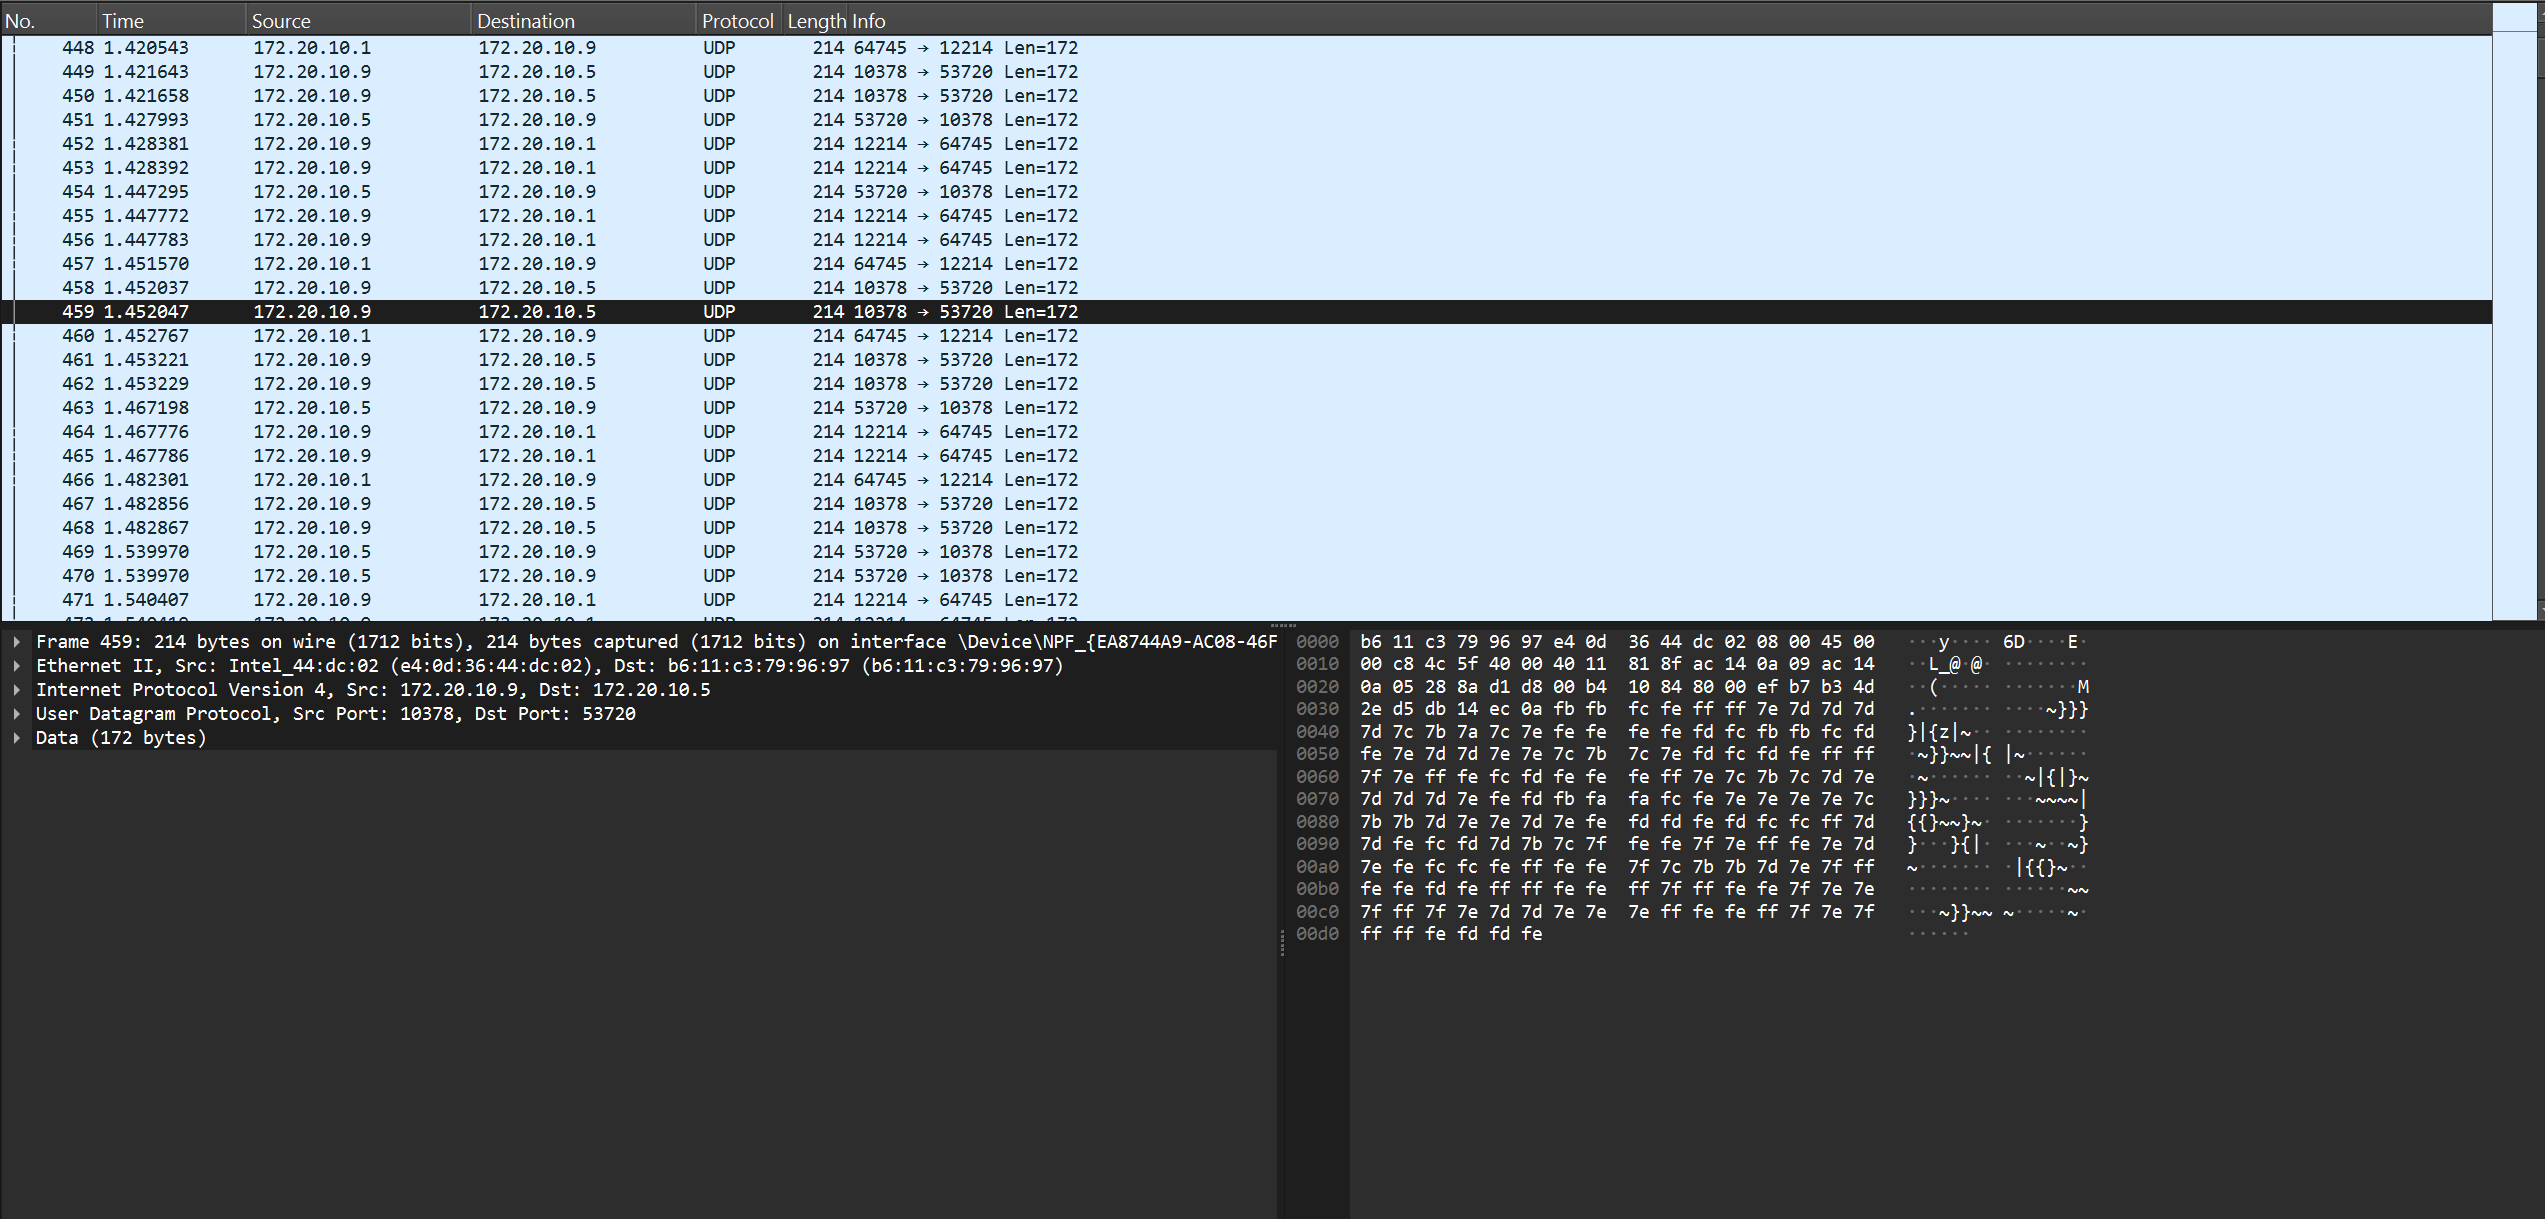
\includegraphics[width=0.95\textwidth]{lab-02-screenshots/8.6-DuranteLlamada.png}
    \caption{Tráfico \textbf{UDP} correspondiente al flujo de voz (posible \textbf{RTP}) en una llamada \textbf{SIP}.}
\end{figure}

\begin{figure}[H]
    \centering
    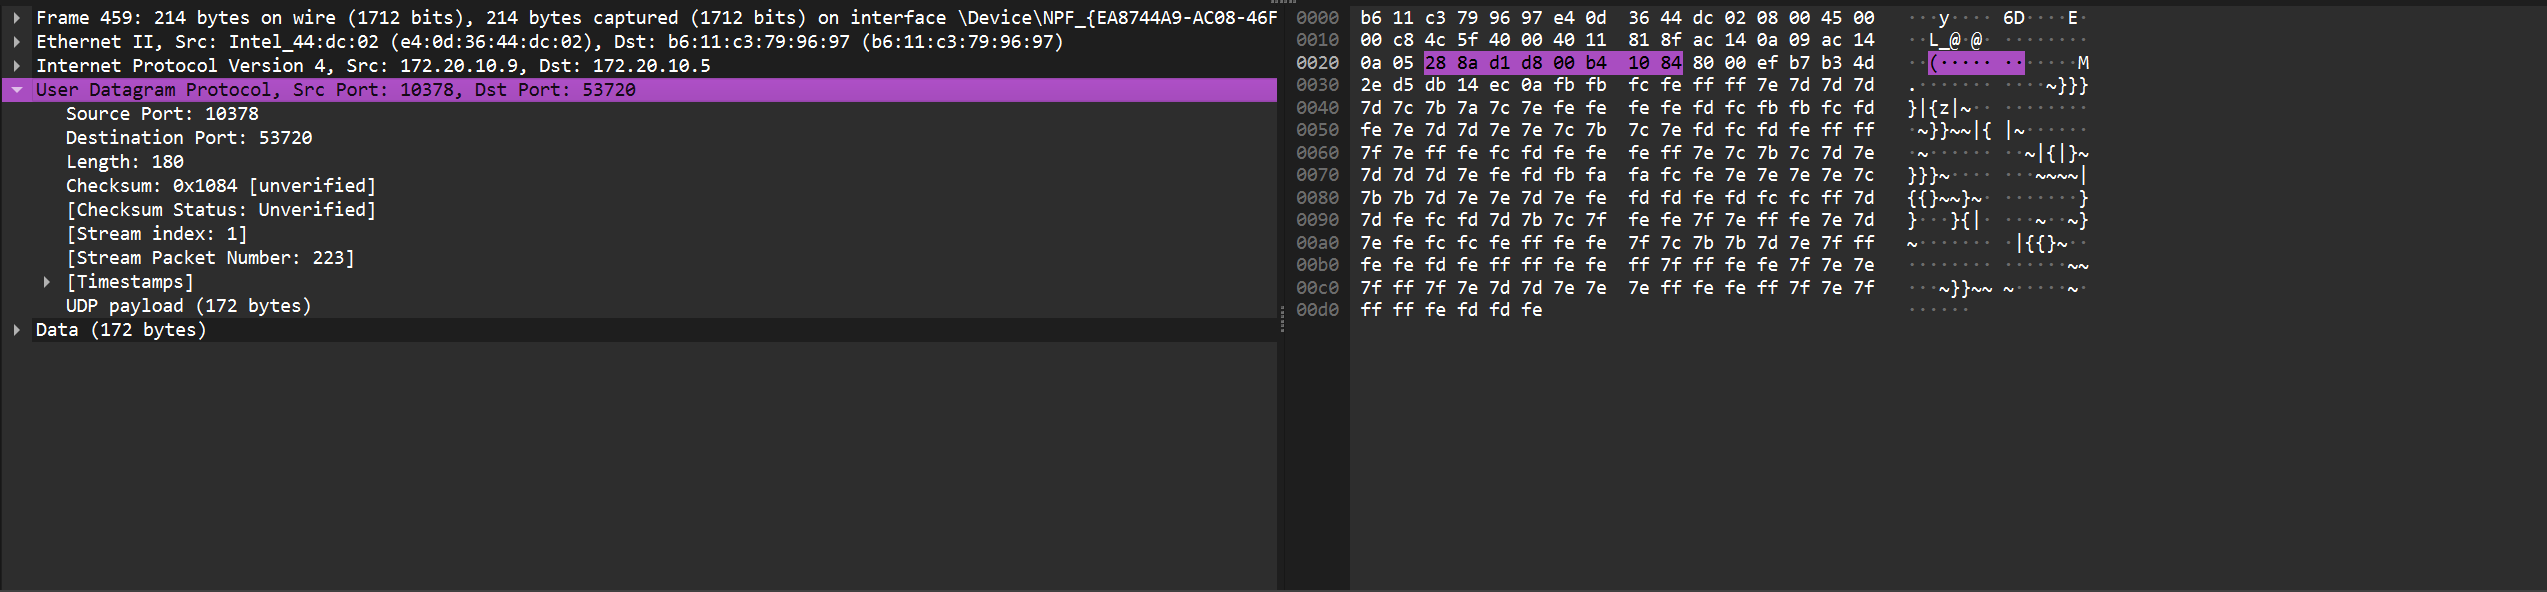
\includegraphics[width=0.95\textwidth]{lab-02-screenshots/8.6-UDPDurante.png}
    \caption{Detalle trafico protocolo \textbf{udp}.}
\end{figure}
A continuacion vemos el detalle de este paquete.
\begin{itemize}
    \item \textbf{Ethernet II}: comunicación entre las direcciones MAC \texttt{e4:0d:36:44:dc:02} (origen) y \texttt{b6:11:c3:79:96:97} (destino).
    \item \textbf{IPv4}: paquete enviado desde \texttt{172.20.10.9} hacia \texttt{172.20.10.5}.
    \item \textbf{UDP}: segmento con puerto de origen \texttt{10378} y puerto de destino \texttt{53720}, longitud de \texttt{180} bytes.
    \item \textbf{Carga útil (172 bytes)}: corresponde al flujo de audio, probablemente un paquete \texttt{RTP} con datos de voz codificados.
\end{itemize}
\subsection*{Conclusiones generales}
\begin{itemize}
\item \textbf{Información de la capa de aplicación:} Para el registro y la gestión de la sesión, se utiliza el protocolo \textbf{SIP} (Session Initiation Protocol), que opera en la capa de aplicación. Este protocolo emplea métodos como \texttt{REGISTER} para autenticar a los clientes y establecer la conexión, y utiliza códigos de estado (similares a HTTP) para indicar el éxito o fracaso de las peticiones.
\item \textbf{Protocolo de la capa de transporte:} Durante el proceso de registro y la transmisión de datos de voz, el protocolo de la capa de transporte utilizado es \textbf{UDP} (User Datagram Protocol). UDP se elige por ser un protocolo sin conexión que prioriza la velocidad sobre la fiabilidad, lo que es ideal para aplicaciones de tiempo real como la voz sobre IP (VoIP), donde una pequeña pérdida de paquetes es preferible a una latencia alta. Además, se menciona que el protocolo \textbf{RTP} (Real-time Transport Protocol), que también utiliza UDP, es el que se encarga de transportar la información de audio durante la llamada.
\item \textbf{Puertos utilizados:} Se identifican los siguientes puertos: el puerto estándar \textbf{5060} se utiliza para la señalización y el registro de clientes a través de SIP, mientras que para el flujo de voz durante la llamada, se utilizan puertos dinámicos. En el ejemplo, el puerto de origen es \textbf{10378} y el de destino es \textbf{53720}.
\end{itemize}
%==============================================================
%=====================   8.7   ================================
%==============================================================
\renewcommand{\thesection}{8.\arabic{section}}
\section{Análisis del protocolo RTMP}
\subsection{Inicio de la transmisión}

Al iniciar la transmision se hace uso del protocolo \textbf{TCP} para establecer conexion entre el servidor y el cliente, esto se hace a traves del uso de las flags (\textit{SYN, ACK} y que de esta manera se establezca el three way handshake y poder proceder con el inicio del protocolo \textbf{RTMP} asi como se puede ver en las siguientes imagenes:

\begin{figure}[H]
    \centering
    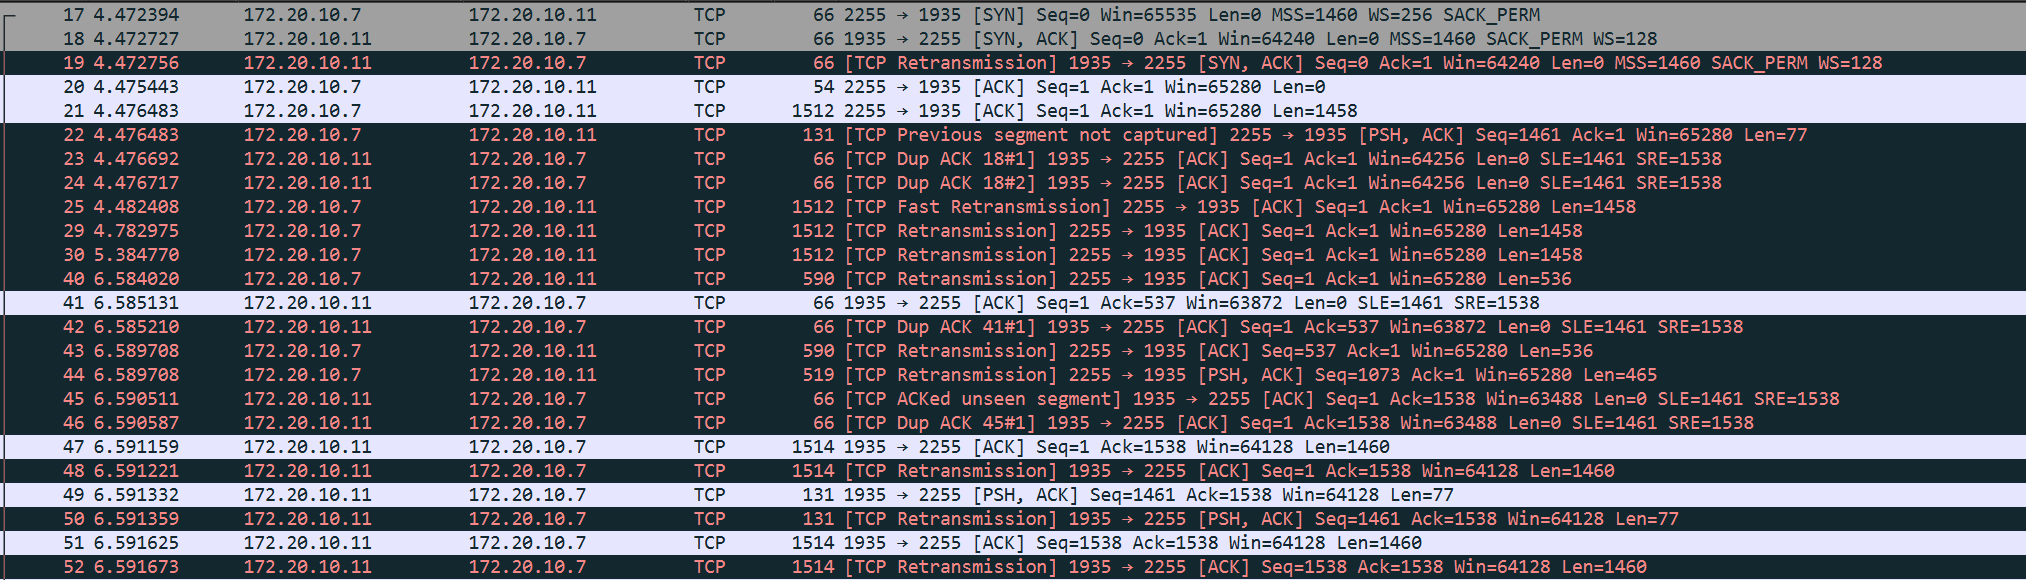
\includegraphics[width=0.95\textwidth]{lab-02-screenshots/8.7-inicioTransmicion.png}
    \caption{Conexion entre el cliente y el servidor usando TCP.}
\end{figure}
\begin{figure}[H]
    \centering
    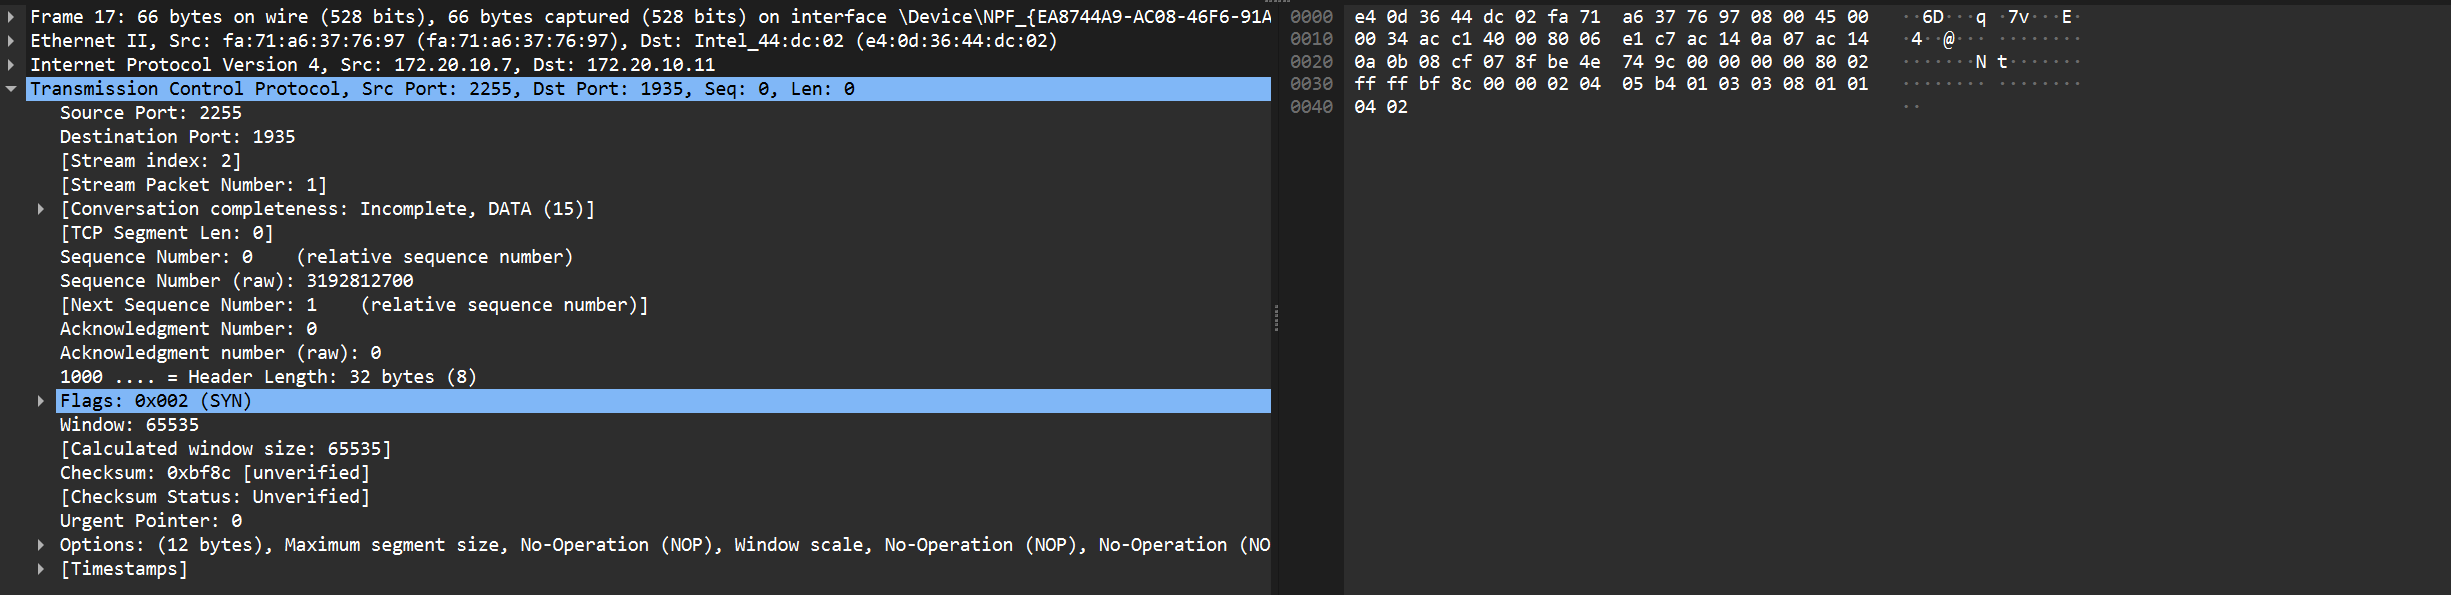
\includegraphics[width=0.95\textwidth]{lab-02-screenshots/8.7-detalleTCP.png}
    \caption{Detalle trafico protocolo \textbf{TCP}.}
\end{figure}

\begin{itemize}
    \item \textbf{Tipo de Paquete:} Es un segmento TCP (Transmission Control Protocol).
    \item \textbf{Inicio de Conexión:} El flag \texttt{SYN} (Synchronize) está activado (marcado como \texttt{0x002}). Esto indica que el cliente está solicitando iniciar una nueva conexión con el servidor.
    \item \textbf{Origen y Destino:} La comunicación se origina desde la dirección IP \texttt{172.28.10.7} en el puerto \texttt{1255} y se dirige a la IP \texttt{172.28.10.11} en el puerto \texttt{1955}.
    \item \textbf{Número de Secuencia:} El número de secuencia inicial es 0, lo cual es típico al comenzar una conexión.
\end{itemize}
En este paquete encontramos la siguiente informacion:
\begin{itemize}
    \item \textbf{Puerto origen:} 2255
    \item \textbf{Puerto destino:} 1935
    \item \textbf{Número de secuencia:} 0 (relativo)
    \item \textbf{Número de acuse:} 0
    \item \textbf{Ventana:} 65535
    \item \textbf{Longitud de cabecera:} 32 bytes
    \item \textbf{Opciones:} MSS, NOP, Window Scale, NOP, NOP
\end{itemize}

\subsection{Conexion Streaming}

Seguido a esto, se inicia la conexión usando el protocolo \textbf{RTMP} (\textit{Real-Time Messaging Protocol}), el cual funciona sobre TCP y está diseñado 
para la transmisión en tiempo real de audio, video y datos a través de internet.  Su función principal es mantener una comunicación estable y de baja latencia entre un cliente y un servidor de medios, permitiendo la transmisión continua (\textit{streaming}) de contenidos multimedia. RTMP fragmenta los datos en mensajes y los envía de manera ordenada, garantizando sincronización y fluidez en la reproducción. A continuacion veremos como funciona segun lo capturado en wireshark:

\begin{figure}[H]
    \centering
    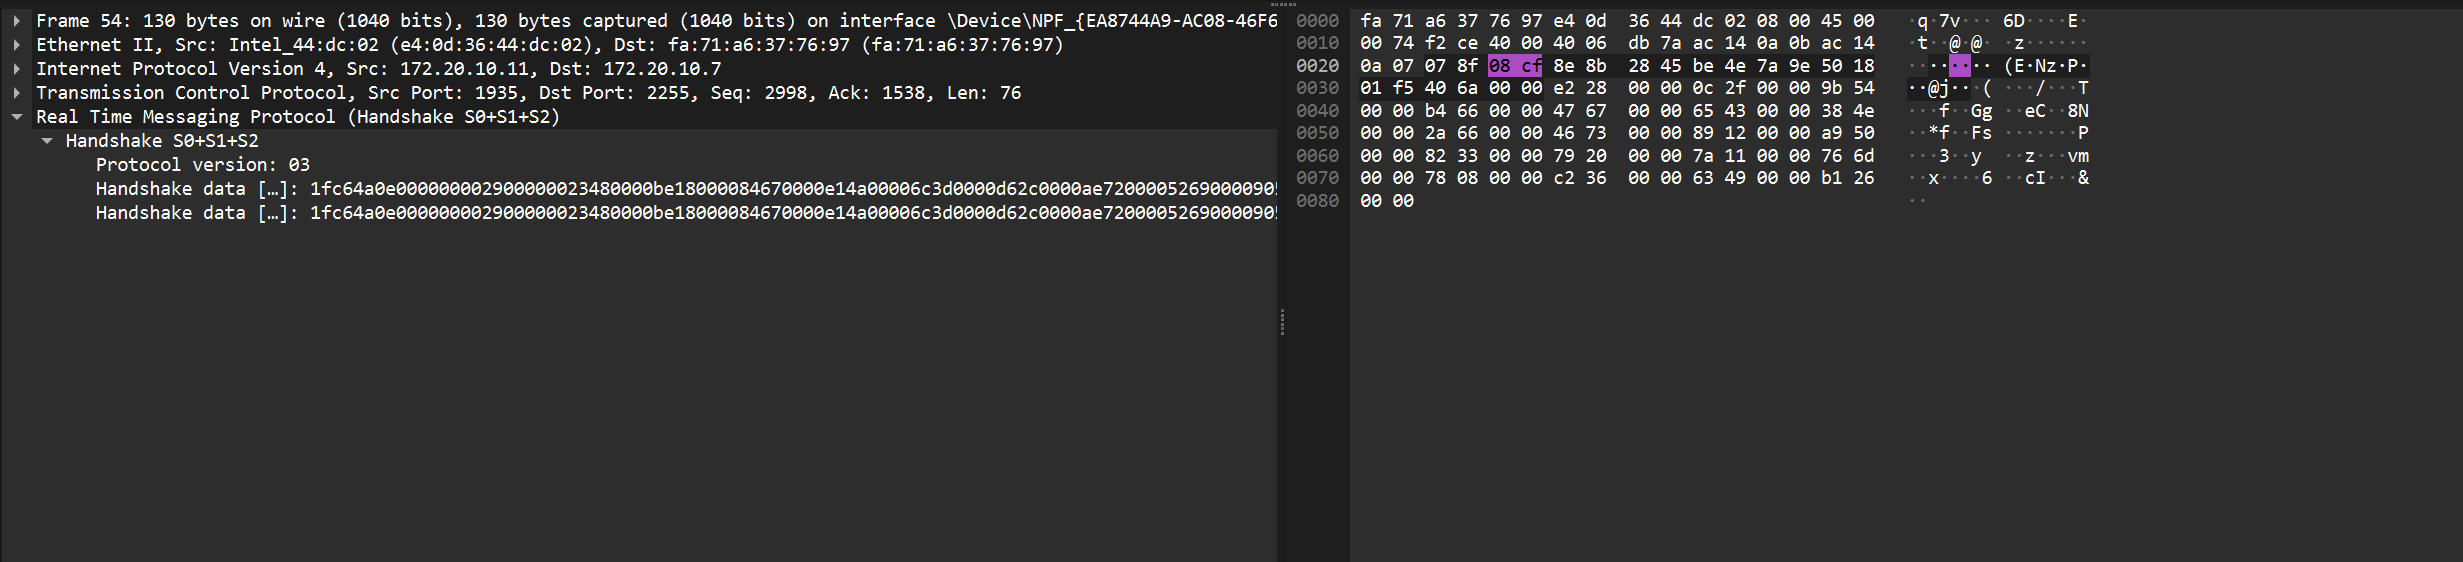
\includegraphics[width=0.95\textwidth]{lab-02-screenshots/8.7-rtmp1.png}
    \caption{Detalle protocolo rtmp inicio.}
\end{figure}
\begin{figure}[H]
    \centering
    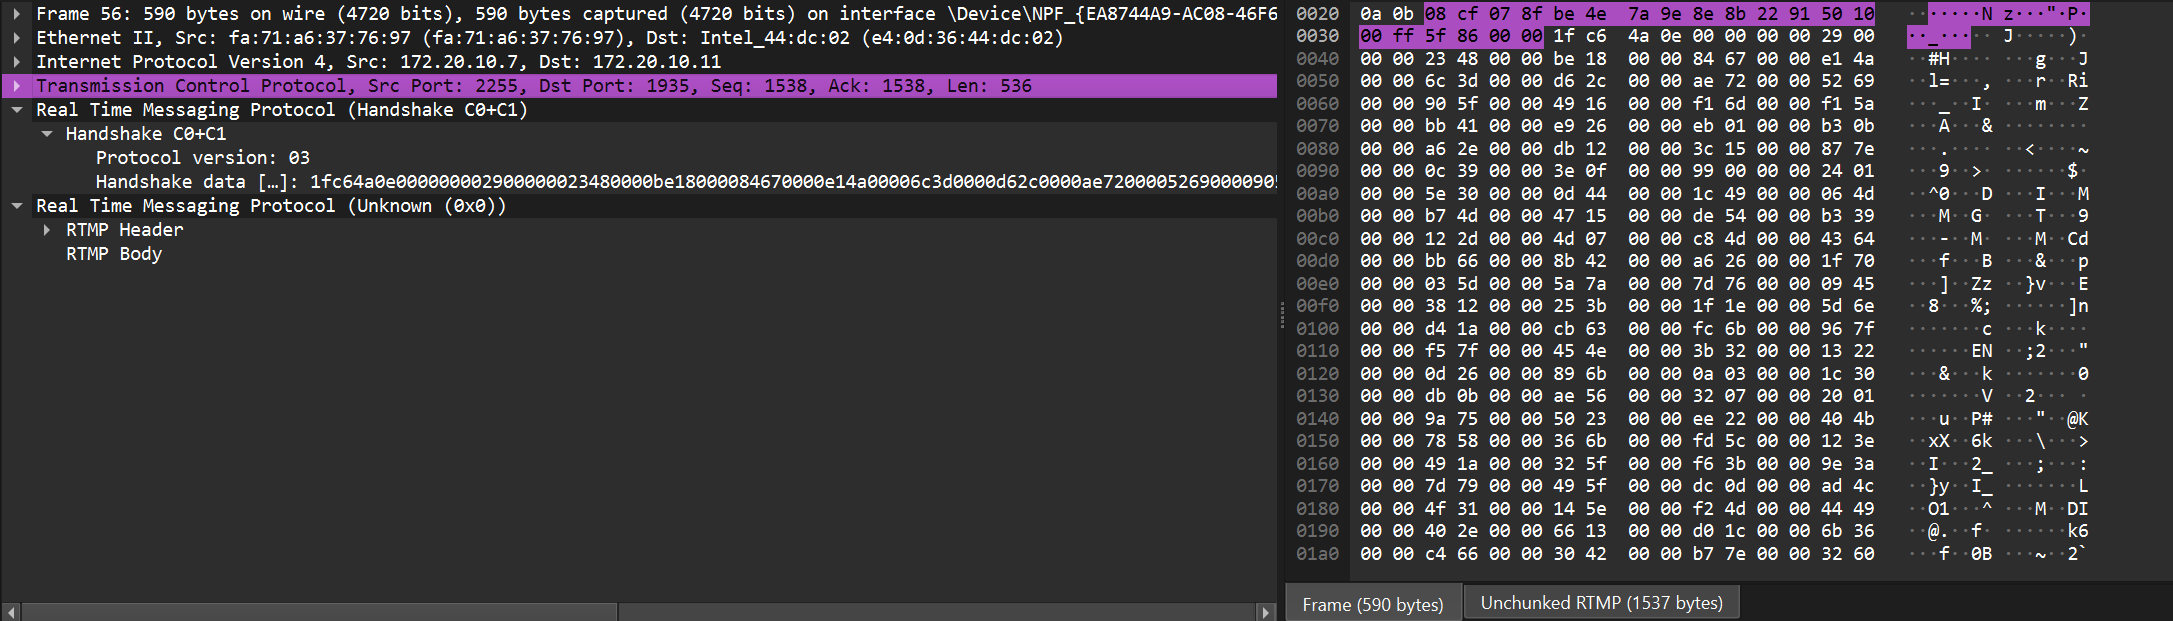
\includegraphics[width=0.95\textwidth]{lab-02-screenshots/8.7-rtmp2.png}
    \caption{Detalle protocolo rtmp durante la transmision.}
\end{figure}
\begin{figure}[H]
    \centering
    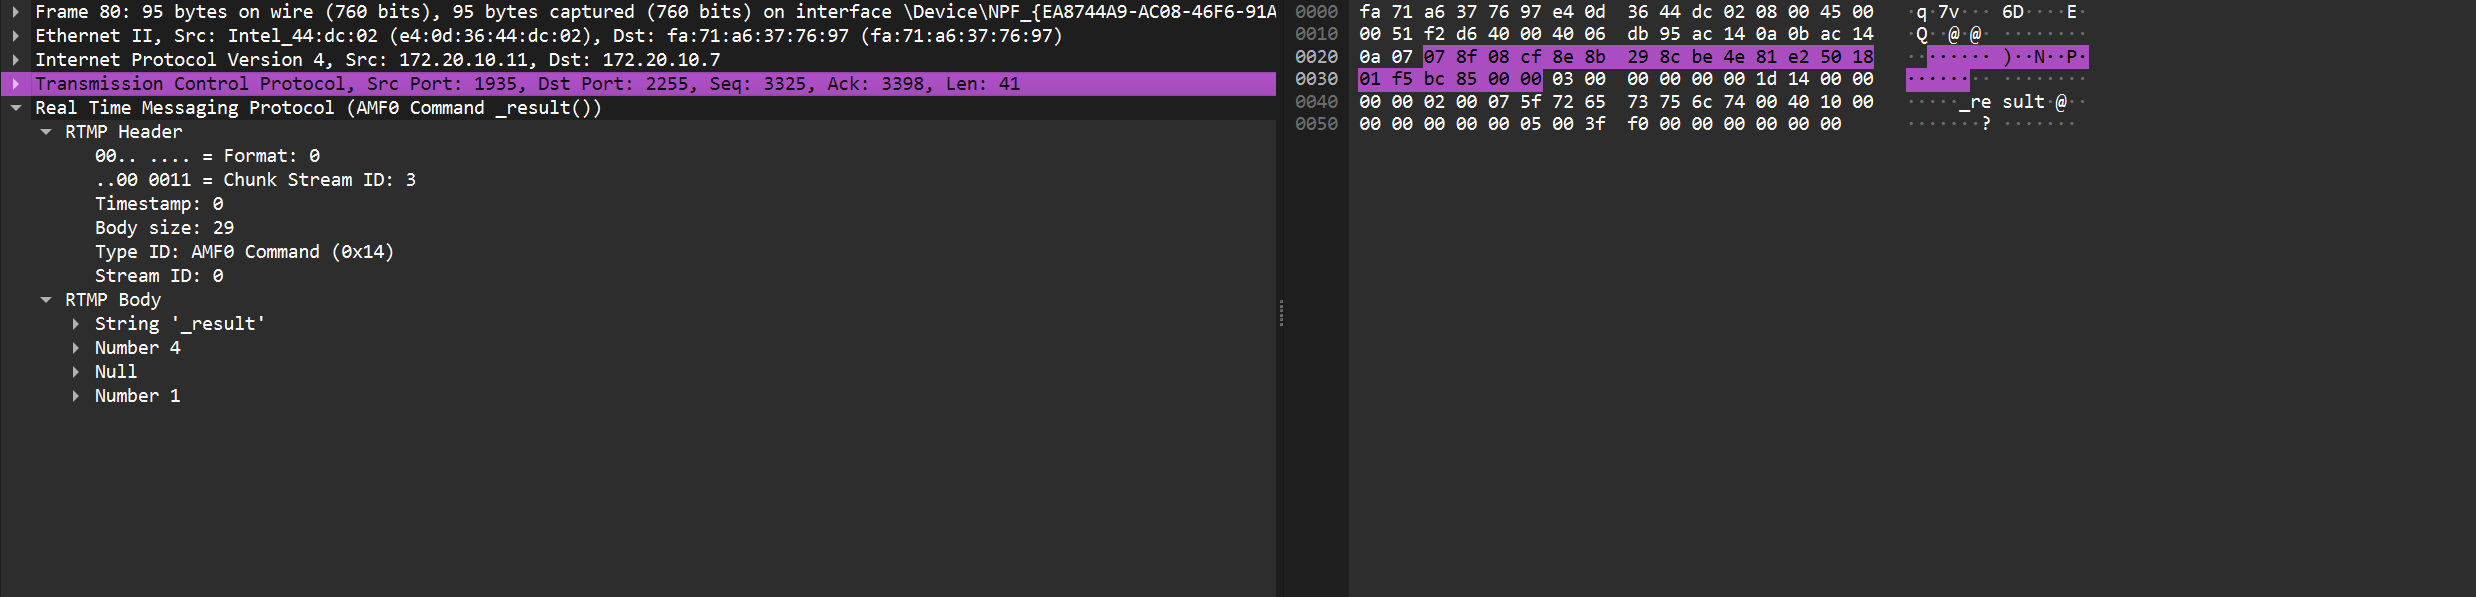
\includegraphics[width=0.95\textwidth]{lab-02-screenshots/8.7-rtmp3.png}
    \caption{Detalle protocolo rtmp durante la transmision.}
\end{figure}

\begin{itemize}
    \item \textbf{Handshake C0+C1:} El cliente envía la versión del protocolo (03) 
    junto con datos de inicialización (timestamp y datos aleatorios).
    \item \textbf{Handshake S0+S1+S2:} El servidor responde confirmando la versión, 
    enviando sus propios datos de inicialización y devolviendo los del cliente.
    \item \textbf{Handshake C2:} El cliente confirma la recepción de los datos del servidor, 
    completando así el proceso de sincronización.
    \item \textbf{RTMP Command (AMF0 \_result):} Una vez finalizado el \textit{handshake}, 
    se intercambian comandos de control en formato AMF0, como la respuesta \_result, 
    que confirma la correcta conexión y preparación del canal para transmitir audio, 
    video y datos en tiempo real.
\end{itemize}
Ahora bien, veamos como va funcionando el flujo de los paquetes durante la transmision:
\begin{figure}[H]
    \centering
    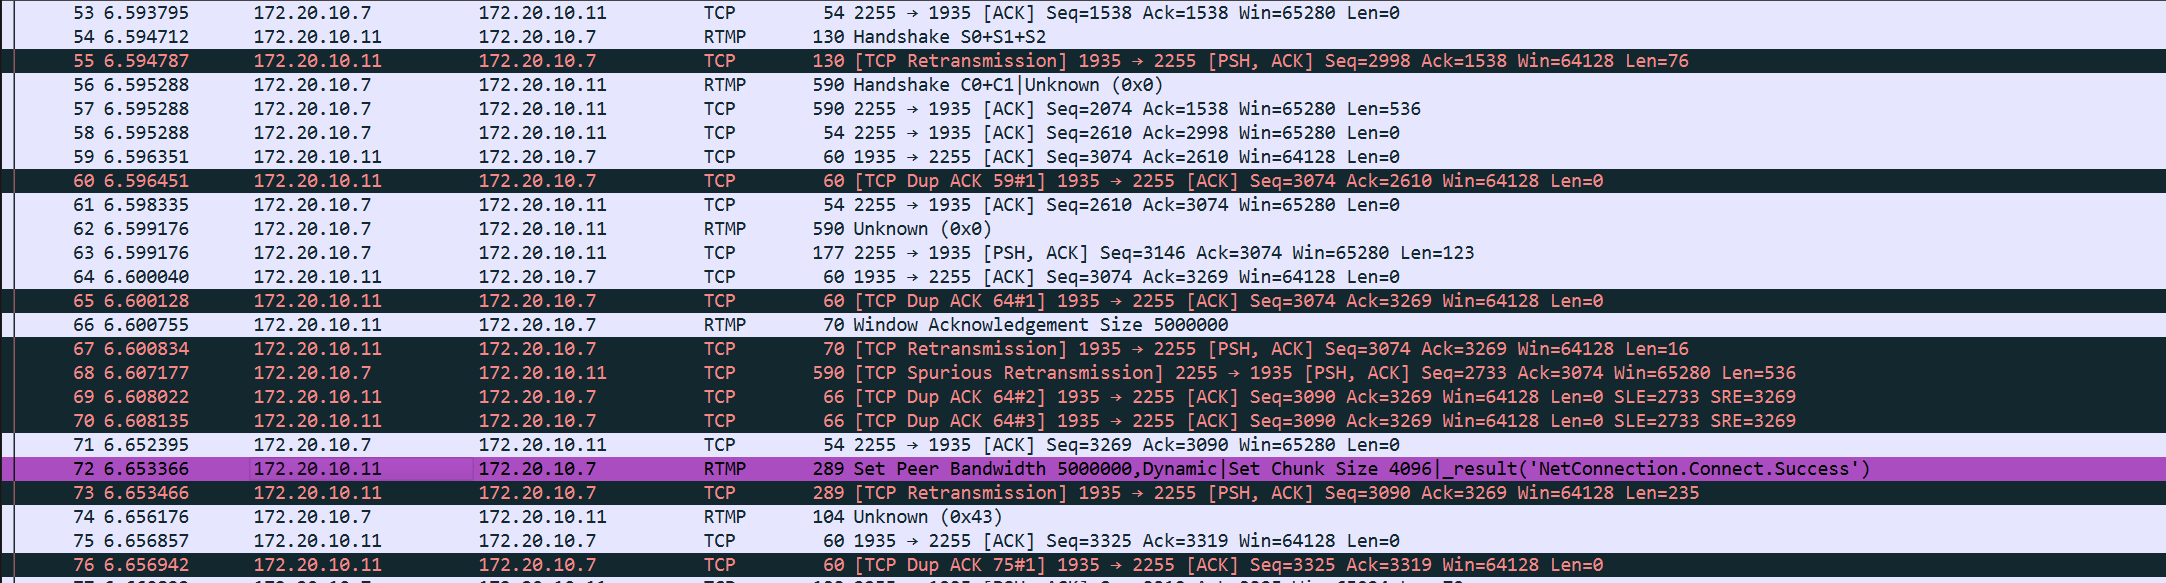
\includegraphics[width=0.95\textwidth]{lab-02-screenshots/8.7-conexionGeneral.png}
    \caption{Detalle protocolo rtmp durante la transmision.}
\end{figure}

Tras completar el \textbf{handshake} inicial de RTMP, se observa el intercambio de mensajes de configuración entre el cliente (172.20.10.7) y el servidor (172.20.10.11), junto con retransmisiones y confirmaciones de control en la capa TCP.  

\begin{itemize}
    \item El cliente envía el \textbf{Handshake C0+C1} y el servidor responde con 
    \textbf{S0+S1+S2}, completando la fase de sincronización.
    \item Se observan varias retransmisiones TCP y \textbf{ACK duplicados}, lo que indica 
    pérdida o retraso de paquetes en la comunicación.
    \item El servidor envía el mensaje \textbf{Window Acknowledgement Size} (5000000), 
    que define el tamaño máximo de ventana para el control de flujo.
    \item Posteriormente, el servidor transmite los comandos 
    \textbf{Set Peer Bandwidth (5000000, Dynamic)} y 
    \textbf{Set Chunk Size (4096)}, que establecen los parámetros de transmisión.
    \item Finalmente, se observa el comando \textbf{\_result('NetConnection.Connect.Success')}, 
    que confirma la conexión exitosa del cliente al servidor RTMP y marca el inicio 
    de la sesión de transmisión de audio, video y datos.
\end{itemize}

Por ultimo, veamos como el protocolo \textbf{RTMP} utiliza el protocolo de la capa de transporte \textbf{RTMP} para mantener una conexion estable y confiable con el servidor:
\begin{figure}[H]
    \centering
    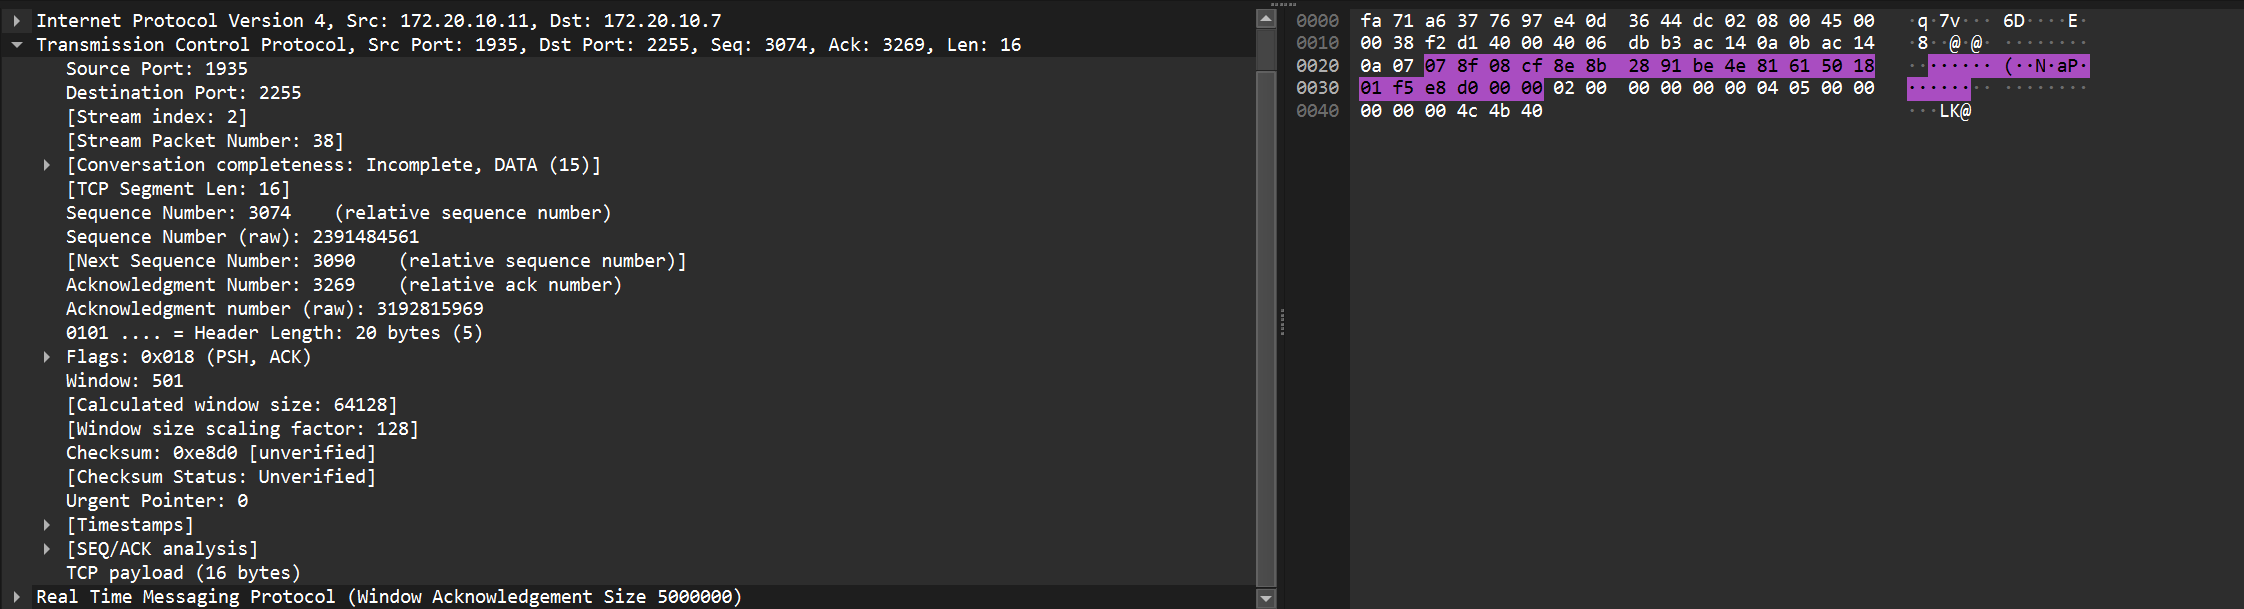
\includegraphics[width=0.95\textwidth]{lab-02-screenshots/8.7-rtmpTCP.png}
    \caption{Detalle protocolo RTMP usando el TCP.}
\end{figure}
\begin{itemize}
    \item El paquete utiliza la bandera \textbf{PSH, ACK}, indicando que 
    los datos deben ser entregados de inmediato a la capa superior.
    \item El payload contiene un mensaje \textbf{Window Acknowledgement Size}, 
    cuyo valor es \textbf{5,000,000 bytes}.
    \item Este parámetro establece el límite máximo de datos que pueden ser 
    enviados antes de requerir una confirmación, permitiendo al servidor 
    regular el flujo de transmisión hacia el cliente.
    \item Forma parte de la negociación de parámetros después del 
    \textbf{handshake RTMP}, y es esencial para el control de congestión 
    y el rendimiento de la sesión de streaming.
\end{itemize}


\subsection*{Conclusion final}

\begin{itemize}
    \item \textbf{Información de la capa de aplicación:} Se identificó el uso del protocolo 
    \textbf{RTMP (Real-Time Messaging Protocol)}, encargado de la transmisión en tiempo real 
    de audio, video y datos, soportado en mensajes como \textit{Handshake}, 
    \textit{Window Acknowledgement Size}, \textit{Set Peer Bandwidth} y 
    \textit{NetConnection.Connect.Success}.
    
    \item \textbf{Protocolo de la capa de transporte:} La transmisión hace uso de 
    \textbf{TCP}, que garantiza una comunicación confiable mediante el 
    \textit{three-way handshake} (SYN, SYN-ACK, ACK), retransmisiones y confirmaciones.
    
    \item \textbf{Puertos utilizados:} El servidor emplea el puerto estándar 
    \textbf{1935} para RTMP, mientras que el cliente se conecta desde un puerto dinámico, 
    identificado en la captura como el \textbf{2255}.
\end{itemize}





\begin{thebibliography}{9}


  \bibitem{kurose_ross}
  Computer Networking, a top-down approach. James Kurose, Keith Ross. Addison-Wesley, 6th ed.

  \end{thebibliography}


\end{document}